\documentclass[11pt, letterpaper]{article}
\usepackage[utf8]{inputenc}
\usepackage[spanish]{babel}
\usepackage{amsmath, amssymb, amsthm}
\usepackage{xcolor}
\usepackage{fancyhdr}
\usepackage{titlesec}
\usepackage[most]{tcolorbox}
\usepackage{enumitem}
\usepackage{graphicx}
\usepackage[margin=2.5cm, top=3cm, bottom=2.5cm]{geometry}

% --- EVITAR ESPACIOS EN BLANCO FORZADOS ---
\raggedbottom 

% --- Definición de Colores ---
\definecolor{azulFES}{RGB}{44, 75, 120}
\definecolor{doradoFES}{RGB}{184, 134, 45}
\definecolor{fondoCaja}{RGB}{246, 248, 250}
\definecolor{bordeCaja}{RGB}{200, 206, 215}
\definecolor{grisTexto}{RGB}{110, 115, 120}
\definecolor{fondoSolucion}{RGB}{250, 252, 255}

% --- Configuración del Encabezado ---
\pagestyle{fancy}
\fancyhf{}
\fancyhead[L]{\textcolor{grisTexto}{Temas Variados de Procesos Estocásticos}}
\fancyhead[R]{\textcolor{grisTexto}{FES Acatlán, UNAM}}
\renewcommand{\headrulewidth}{0.5pt}
\renewcommand{\headrule}{\hbox to\headwidth{\color{bordeCaja}\leaders\hrule height \headrulewidth\hfill}}

% --- Configuración de Títulos ---
\titleformat{\section}{\normalfont\Large\bfseries\color{azulFES}}{\thesection.}{1em}{}[{\vspace{2mm}\color{doradoFES}\titlerule[1.5pt]}]

% --- Cajas (Con 'breakable' para evitar espacios en blanco) ---
\newtcolorbox{ejercicio}{
  colback=fondoCaja, colframe=bordeCaja, boxrule=0.8pt, arc=4pt,
  left=10pt, right=10pt, top=10pt, bottom=10pt, parbox=false,
  before skip=12pt, after skip=0pt, breakable
}

\newtcolorbox{solucion}{
  colback=fondoSolucion, colframe=azulFES, colbacktitle=azulFES,
  title=\textbf{Solución}, fonttitle=\bfseries,
  boxrule=0.8pt, arc=4pt,
  left=10pt, right=10pt, top=10pt, bottom=10pt, parbox=false,
  before skip=0pt, after skip=12pt, breakable
}

\setlist[enumerate,1]{label=(\alph*)}

\begin{document}

% ==========================================
%                 PORTADA
% ==========================================
\begin{titlepage}
    \centering
    % Descomenta la siguiente línea si tienes el logo en la misma carpeta
    
\includegraphics[width=0.45\textwidth]{UNAM (1).png} \\
    \vspace{1cm}
    
    {\Large \textbf{Universidad Nacional Autónoma de México}} \\
    \vspace{0.1cm}
    {\large \textbf{Facultad de Estudios Superiores Acatlán}} \\
    \vspace{0.1cm}
    {\large División de Matemáticas e Ingeniería} \\
    \vspace{0.1cm}
    {\large Licenciatura en Matemáticas Aplicadas y Computación} \\
    \vspace{1.5cm}
    
    {\large \textbf{Nombre:} Emiliano Ruiz Sánchez} \\
    \vspace{0.5cm}
            
    {\large \textbf{Materia:} Procesos Estocásticos} \\
    \vspace{0.1cm}
    {\large \textbf{Tema:} Cadenas de Markov a tiempo continuo, Proceso de Poisson, Colas
Optimal Stopping, Martingalas y Cambios de Medida
} \\
    \vspace{0.5cm}
    \vfill
\end{titlepage}

\newpage

% ==========================================
%                 BLOQUE 1
% ==========================================
\section{Cadenas de Markov a tiempo continuo: generador, construcción y ergodicidad}

\begin{ejercicio}
\textbf{EJERCICIO 1.1.} Sea $(X_{t})_{t\ge0}$ una cadena de Markov a tiempo continuo sobre un espacio numerable $S$ con semigrupo $(P_{t})_{t>0}$. Suponga que para toda función acotada $f:S\rightarrow\mathbb{R}$ existe el límite 
\[ Lf(x):=\lim_{t\downarrow 0}\frac{P_{t}f(x)-f(x)}{t} \] 
Demuestre que $L$ es lineal y que, para la familia de indicadores $1_{\{y\}}$, se tiene 
\[ L1_{\{y\}}(x)=\alpha(x,y) \quad (y\ne x), \quad L1_{\{x\}}(x)=A(x,x)=-\alpha(x). \] 
Concluya que existe una familia de coeficientes $\alpha(x,y)$, para $y\ne x$ tal que $\alpha(x,y)\ge0$ y que la matriz generadora infinitesimal $A$ viene dada por $A(x,y)=\alpha(x,y)$ si $y\ne x$ y $A(x,x)=-\alpha(x)$, donde $\alpha(x)=\sum_{y\ne x}\alpha(x,y)$. Interprete estos coeficientes en términos de tasas instantáneas de salto. 
\end{ejercicio}
\begin{solucion}
    \textbf{Linealidad de $L$:} Sean $f, g$ funciones acotadas y $c \in \mathbb{R}$. Por la linealidad de la esperanza condicional (y del operador $P_t$), tenemos $P_t(cf + g)(x) = cP_tf(x) + P_tg(x)$. Entonces:
    \begin{align*}
        L(cf+g)(x) &= \lim_{t\downarrow 0} \frac{P_t(cf+g)(x) - (cf(x)+g(x))}{t} \\
        &= c \lim_{t\downarrow 0} \frac{P_tf(x)-f(x)}{t} + \lim_{t\downarrow 0} \frac{P_tg(x)-g(x)}{t} = cLf(x) + Lg(x).
    \end{align*}
    
    \textbf{Evaluación en funciones indicadoras:} Consideremos $f(z) = 1_{\{y\}}(z)$. Notemos que $P_t 1_{\{y\}}(x) = \mathbb{E}_x[1_{\{y\}}(X_t)] = \mathbb{P}_x(X_t = y) = p_t(x,y)$. 
    Si $y \neq x$, $1_{\{y\}}(x) = 0$, por lo que:
    \[ L1_{\{y\}}(x) = \lim_{t\downarrow 0} \frac{p_t(x,y) - 0}{t} =: \alpha(x,y) = A(x,y). \]
    Puesto que $p_t(x,y) \ge 0$ para $t > 0$, se sigue que $\alpha(x,y) \ge 0$. \\
    Para $y = x$, $1_{\{x\}}(x) = 1$, entonces:
    \[ L1_{\{x\}}(x) = \lim_{t\downarrow 0} \frac{p_t(x,x) - 1}{t} =: -\alpha(x) = A(x,x). \]
    Dado que $\sum_{y \in S} p_t(x,y) = 1$, al derivar respecto a $t$ en $t=0$ obtenemos $\sum_{y \in S} A(x,y) = 0$, lo que implica $A(x,x) = -\sum_{y \neq x} A(x,y)$, es decir, $\alpha(x) = \sum_{y \neq x} \alpha(x,y)$.
    
    \textbf{Interpretación:} Los coeficientes $\alpha(x,y)$ representan la \textit{tasa instantánea} a la cual la cadena salta del estado $x$ al estado $y$. Por su parte, $\alpha(x)$ es la tasa total de salida del estado $x$.
\end{solucion}

\begin{ejercicio}
\textbf{EJERCICIO 1.2.} Sea $A$ una matriz generadora infinitesimal conservativa sobre un conjunto numerable $S$. Muestre que si una cadena de Markov a tiempo continuo con generador $A$ existe y es no explosiva, entonces para todo estado $x$ el tiempo de permanencia en $x$ tiene ley exponencial de parámetro $\alpha(x)$, y condicionado al evento de que ocurra un salto desde $x$, la distribución del siguiente estado viene dada por 
\[ \mathbb{P}_{x}(X_{T_{1}}=y|T_{1}<\infty)=r(x,y)=\frac{\alpha(x,y)}{\alpha(x)}, \quad y\ne x. \] 
Concluya que la cadena puede construirse a partir de tiempos exponenciales y de la cadena embebida. 
\end{ejercicio}
\begin{solucion}
    Sea $T_1 = \inf\{t > 0 : X_t \neq x\}$ el tiempo de permanencia en el estado inicial $x$. Por la propiedad de Markov fuerte (o pérdida de memoria de la cadena a tiempo continuo), la probabilidad de permanecer en $x$ un tiempo adicional $s$ dado que ya se ha permanecido un tiempo $t$ es independiente de $t$:
    \[ \mathbb{P}_x(T_1 > t + s \mid T_1 > t) = \mathbb{P}_x(T_1 > s). \]
    La única distribución continua no negativa con esta propiedad es la exponencial. La tasa de abandono del estado $x$ está dada por el generador infinitesimal en la diagonal, es decir, $\lim_{h \to 0} \frac{1 - \mathbb{P}_x(T_1 > h)}{h} = -A(x,x) = \alpha(x)$. Así, $T_1 \sim \text{Exp}(\alpha(x))$.
    
    Para determinar el estado de destino al ocurrir el salto, sabemos que en un intervalo de tiempo pequeño $h$, la probabilidad de saltar a $y$ es $\alpha(x,y)h + o(h)$. La probabilidad de abandonar $x$ en ese mismo intervalo es $\alpha(x)h + o(h)$. Por definición de probabilidad condicional:
    \[ \mathbb{P}_x(X_{T_1} = y \mid T_1 \le h) = \frac{\alpha(x,y)h + o(h)}{\alpha(x)h + o(h)} \xrightarrow{h \to 0} \frac{\alpha(x,y)}{\alpha(x)} = r(x,y). \]
    Dado que la cadena no es explosiva (hace un número finito de saltos en tiempo finito casi seguramente), podemos construirla iterativamente: estando en $x$, muestreamos el tiempo de permanencia con $E \sim \text{Exp}(\alpha(x))$ y, de forma independiente, elegimos el siguiente estado $y$ según la distribución de la cadena discreta embebida $r(x,y)$.
\end{solucion}

\begin{ejercicio}
\textbf{EJERCICIO 1.3.} (Sistema de inventario.) Una tienda mantiene un inventario $X_{t}\in\mathbb{N}_{0}$ de cierto artículo. Las llegadas de nuevos pedidos del proveedor ocurren a tasa constante $\lambda$ y las ventas a clientes ocurren a tasa $\mu$ mientras haya existencia disponible. Modele $(X_{t})_{t\ge0}$ como una cadena nacimiento-muerte sobre $\mathbb{N}_{0}$ con tasas 
\[ \alpha(n,n+1)=\lambda, \quad \alpha(n,n-1)=\mu 1_{\{n\ge1\}}. \] 
Escriba explícitamente las ecuaciones de Kolmogorov hacia adelante y hacia atrás para las probabilidades $p_{t}(i,j)$. Aplique sus fórmulas para derivar el sistema diferencial satisfecho por $m_{i}(t):=\mathbb{E}_{i}[X_{t}]$ e interprete el signo de $m_{i}^{\prime}(t)$ según la relación entre $\lambda$ y $\mu$. 
\end{ejercicio}
\begin{solucion}
    Las ecuaciones de \textbf{Kolmogorov hacia adelante} (Forward) $P'(t) = P(t)A$ nos dan las derivadas respecto al estado de llegada $j$:
    \begin{align*}
        p_t'(i,0) &= -\lambda p_t(i,0) + \mu p_t(i,1) \\
        p_t'(i,j) &= \lambda p_t(i,j-1) - (\lambda + \mu) p_t(i,j) + \mu p_t(i,j+1), \quad \text{para } j \ge 1.
    \end{align*}
    
    Las ecuaciones de \textbf{Kolmogorov hacia atrás} (Backward) $P'(t) = AP(t)$ nos dan las derivadas respecto al estado inicial $i$:
    \begin{align*}
        p_t'(0,j) &= -\lambda p_t(0,j) + \lambda p_t(1,j) \\
        p_t'(i,j) &= \mu p_t(i-1,j) - (\lambda + \mu) p_t(i,j) + \lambda p_t(i+1,j), \quad \text{para } i \ge 1.
    \end{align*}

    Para derivar el sistema para $m_i(t) = \mathbb{E}_i[X_t] = \sum_{j=0}^{\infty} j p_t(i,j)$, derivamos bajo el signo de la suma y usamos las ecuaciones hacia adelante:
    \begin{align*}
        m_i'(t) &= \sum_{j=1}^{\infty} j p_t'(i,j) = \sum_{j=1}^{\infty} j \big[ \lambda p_t(i,j-1) - (\lambda + \mu) p_t(i,j) + \mu p_t(i,j+1) \big] \\
        &= \lambda \sum_{k=0}^{\infty} (k+1) p_t(i,k) - (\lambda+\mu) \sum_{j=1}^{\infty} j p_t(i,j) + \mu \sum_{k=2}^{\infty} (k-1) p_t(i,k) \\
        &= \lambda (m_i(t) + 1) - (\lambda+\mu)m_i(t) + \mu (m_i(t) - \mathbb{P}_i(X_t \ge 1)) \\
        &= \lambda - \mu \mathbb{P}_i(X_t \ge 1).
    \end{align*}
    \textbf{Interpretación:} El inventario promedio crece a tasa $\lambda$ y decrece a tasa $\mu$ solo cuando hay inventario ($\mathbb{P}_i(X_t \ge 1)$). 
    Si $\lambda > \mu$, entonces $m_i'(t) \ge \lambda - \mu > 0$, el inventario esperado crecerá indefinidamente hacia el infinito. Si $\lambda < \mu$, el inventario esperado tenderá a estabilizarse, ya que cuando se acerca a 0, la probabilidad $\mathbb{P}_i(X_t \ge 1)$ se ajusta para que la derivada se anule.
\end{solucion}

\begin{ejercicio}
\textbf{EJERCICIO 1.4.} Sea $X$ una cadena irreducible sobre un espacio finito $S$ con generador $A$. Demuestre que existe una única distribución invariante $\pi$ y que toda solución del sistema lineal 
\[ \pi A=0, \quad \sum_{x\in S}\pi(x)=1 \] 
coincide con dicha medida invariante. Pruebe además que $\lim_{t\rightarrow\infty}P_{t}(x,y)=\pi(y)$ para todos $x,y\in S$. 
\end{ejercicio}
\begin{solucion}
    Por definición, la matriz generadora $A$ satisface que la suma de cada renglón es cero ($A\mathbf{1} = \mathbf{0}$). Por lo tanto, $\lambda = 0$ es un eigenvalor derecho de $A$ con eigenvector $\mathbf{1}$. Como $S$ es finito e irreducible, el Teorema de Perron-Frobenius (adaptado a generadores $A = P - I$ o mediante la exponencial $P_t = e^{tA}$) asegura que la multiplicidad algebraica de $0$ es $1$. Esto garantiza la existencia de un único eigenvector izquierdo $\pi$ tal que $\pi A = 0$ normalizado tal que $\sum_{x} \pi(x) = 1$. Toda distribución invariante satisface $\frac{d}{dt} \pi P_t = \pi P_t A = 0 \implies \pi A = 0$, por lo que la solución al sistema es única y es la medida invariante.

    Para el comportamiento asintótico, como $S$ es finito e irreducible, la cadena es automáticamente recurrente positiva. Para cualquier $t > 0$, todas las entradas de $P_t = e^{tA}$ son estrictamente positivas (no hay problemas de periodicidad en cadenas a tiempo continuo). Por el Teorema Ergódico para cadenas de Markov a tiempo continuo, se sigue directamente que la matriz de transición asintótica existe y todas sus filas convergen a la distribución estacionaria única:
    \[ \lim_{t\to\infty} P_t(x,y) = \pi(y), \quad \forall x, y \in S. \]
\end{solucion}

\begin{ejercicio}
\textbf{EJERCICIO 1.5.} Sea $X$ una cadena irreducible sobre un espacio numerable $S$ con generador $A$. Suponga que existe una probabilidad $\pi$ tal que 
\[ \pi(x)\alpha(x,y)=\pi(y)\alpha(y,x), \quad x,y\in S, \; x\ne y. \] 
Demuestre que $\pi$ es invariante. Muestre después que, para toda función acotada $f,g:S\rightarrow\mathbb{R}$ y todo $t\ge0$ 
\[ \sum_{x\in S}\pi(x)f(x)P_{t}g(x)=\sum_{x\in S}\pi(x)g(x)P_{t}f(x), \] 
esto es, que el semigrupo es autoadjunto en $L^{2}(\pi)$. Interprete esta propiedad como reversibilidad. 
\end{ejercicio}
\begin{solucion}
    Primero demostramos que $\pi$ es invariante comprobando que $\pi A = 0$. Evaluamos la componente $y$:
    \[ (\pi A)(y) = \sum_{x \in S} \pi(x)A(x,y) = \pi(y)A(y,y) + \sum_{x \neq y} \pi(x)\alpha(x,y). \]
    Por la condición de balance detallado, sustituimos $\pi(x)\alpha(x,y) = \pi(y)\alpha(y,x)$:
    \[ (\pi A)(y) = \pi(y)A(y,y) + \sum_{x \neq y} \pi(y)\alpha(y,x) = \pi(y) \left[ A(y,y) + \alpha(y) \right] = \pi(y) [0] = 0. \]
    Por lo tanto, $\pi$ es invariante.

    Para ver que es autoadjunto, consideremos el producto interno en $L^2(\pi)$, $\langle u, v \rangle_\pi = \sum_{x} \pi(x)u(x)v(x)$. La ecuación de balance detallado equivale a decir que el generador $A$ es un operador autoadjunto: $\langle f, Ag \rangle_\pi = \langle Af, g \rangle_\pi$.
    Dado que el semigrupo está dado formalmente por $P_t = e^{tA} = \sum_{n=0}^{\infty} \frac{t^n A^n}{n!}$, y como $A$ es autoadjunto, cualquier potencia de $A$ lo es, y por lo tanto $P_t$ hereda esta propiedad:
    \[ \langle f, P_t g \rangle_\pi = \langle P_t f, g \rangle_\pi \implies \sum_{x\in S}\pi(x)f(x)P_{t}g(x)=\sum_{x\in S}\pi(x)g(x)P_{t}f(x). \]
    
    \textbf{Interpretación:} Esta es la definición de reversibilidad en el tiempo. Significa que si iniciamos la cadena con la distribución estacionaria $\pi$ y la observamos transcurrir en el sentido inverso del tiempo, la ley de las trayectorias es indistinguible de la ley de la cadena marchando hacia adelante en el tiempo.
\end{solucion}

\begin{ejercicio}
\textbf{EJERCICIO 1.6.} Sea $X$ una cadena irreducible y positiva recurrente sobre un espacio numerable $S$ con medida invariante $\pi$. Demuestre, bajo las hipótesis necesarias que usted formule con precisión, el teorema ergódico 
\[ \frac{1}{t}\int_{0}^{t}f(X_{s})ds \xrightarrow[t\rightarrow\infty]{a.s.} \sum_{x\in S}f(x)\pi(x) \] 
para toda función $f$ integrable respecto de $\pi$. Después aplíquelo al caso de una cadena nacimiento-muerte reversible e interprete el resultado como promedio temporal de un sistema observado durante mucho tiempo. 
\end{ejercicio}
\begin{solucion}
    \textbf{Hipótesis y Demostración:} Supongamos que la cadena es conservativa y no explosiva, y que inicia en el estado $x_0 \in S$. Sea $R_1, R_2, \dots$ la sucesión de tiempos de retorno al estado $x_0$. Como es positiva recurrente, el tiempo medio entre retornos $\mathbb{E}[R_{i+1} - R_i] = \mu_{x_0} < \infty$. 
    Sea $Y_i = \int_{R_{i-1}}^{R_i} f(X_s) ds$. Por la propiedad fuerte de Markov, $\{Y_i\}_{i\ge 2}$ son variables aleatorias i.i.d. 
    Definimos el número de retornos a $x_0$ antes de $t$ como $N(t)$. Entonces podemos acotar la integral:
    \[ \sum_{i=1}^{N(t)} Y_i \le \int_{0}^{t} f(X_s) ds \le \sum_{i=1}^{N(t)+1} Y_i. \]
    Dividiendo entre $t = \frac{t}{N(t)} N(t)$:
    \[ \frac{N(t)}{t} \frac{1}{N(t)}\sum_{i=1}^{N(t)} Y_i \le \frac{1}{t}\int_{0}^{t} f(X_s) ds \le \frac{N(t)+1}{t} \frac{1}{N(t)+1}\sum_{i=1}^{N(t)+1} Y_i. \]
    Por la Ley Fuerte de los Grandes Números, $\frac{1}{N(t)}\sum Y_i \xrightarrow{a.s.} \mathbb{E}[Y_2]$. Por teoría de renovación, $\frac{N(t)}{t} \xrightarrow{a.s.} \frac{1}{\mu_{x_0}}$. 
    Por consiguiente, el límite a.s. es $\frac{\mathbb{E}_{x_0}[\int_0^{R_1} f(X_s) ds]}{\mu_{x_0}}$. 
    Sabemos que la medida invariante satisface $\pi(x) = \frac{1}{\mu_{x_0}} \mathbb{E}_{x_0}\left[\int_0^{R_1} 1_{\{X_s = x\}} ds\right]$, por lo que por linealidad para $f$ $\pi$-integrable, el límite es exactamente $\sum_{x} f(x)\pi(x)$.

    \textbf{Aplicación a Cadena Nacimiento-Muerte:} En una cadena nacimiento-muerte reversible, si evaluamos la función $f(x) = x$, el teorema nos indica que el límite casi seguro de $\frac{1}{t}\int_0^t X_s ds$ será $\sum_{x=0}^\infty x \pi(x)$, la cual es la esperanza del sistema estacionario. 
    \textbf{Interpretación:} El comportamiento promedio de un sistema (como la longitud de una cola o inventario) a lo largo del tiempo para una sola trayectoria (promedio temporal) convergerá, si se observa lo suficiente, al promedio de ensamble teórico del sistema en equilibrio (promedio espacial).
\end{solucion}

\begin{ejercicio}
\textbf{EJERCICIO 1.7.} Considere la caminata aleatoria continua sobre $\mathbb{Z}$ con tasas 
\[ \alpha(x,x+1)=\alpha, \quad \alpha(x,x-1)=\beta, \quad \alpha,\beta>0. \] 
Pruebe que $X_{t}=N_{t}^{+}-N_{t}^{-}$, donde $N^{+}$ y $N^{-}$ son procesos de Poisson independientes de parámetros $\alpha$ y $\beta$, respectivamente. Calcule $\mathbb{E}[X_{t}]$, $\text{Var}(X_{t})$ y la función característica de $X_{t}$. Determine para qué valores de $\alpha, \beta$ puede existir una medida invariante finita. 
\end{ejercicio}
\begin{solucion}
    Dado que las tasas de salto hacia la derecha ($\alpha$) y a la izquierda ($\beta$) no dependen del estado actual $x$, los tiempos entre saltos a la derecha son exponenciales independientes con parámetro $\alpha$ y los de la izquierda con parámetro $\beta$. Por definición, el conteo acumulado de dichos eventos forma dos procesos de Poisson independientes $N_t^+ \sim \text{Poisson}(\alpha t)$ y $N_t^- \sim \text{Poisson}(\beta t)$. Al iniciar en $X_0=0$, la posición en tiempo $t$ es sumar $+1$ por cada salto derecho y $-1$ por cada izquierdo, esto es, $X_t = N_t^+ - N_t^-$.

    \textbf{Momentos:}
    \begin{align*}
        \mathbb{E}[X_t] &= \mathbb{E}[N_t^+] - \mathbb{E}[N_t^-] = \alpha t - \beta t = (\alpha - \beta)t. \\
        \text{Var}(X_t) &= \text{Var}(N_t^+) + \text{Var}(N_t^-) \quad \text{(por independencia)} = \alpha t + \beta t = (\alpha + \beta)t.
    \end{align*}

    \textbf{Función característica:} $\phi_{X_t}(u) = \mathbb{E}[e^{iuX_t}] = \mathbb{E}[e^{iuN_t^+}] \mathbb{E}[e^{-iuN_t^-}]$. Sabiendo la función característica de la Poisson:
    \[ \phi_{X_t}(u) = \exp(\alpha t (e^{iu} - 1)) \exp(\beta t (e^{-iu} - 1)) = \exp\left( t \big[ \alpha(e^{iu}-1) + \beta(e^{-iu}-1) \big] \right). \]

    \textbf{Medida invariante finita:} Para buscar la invariante, necesitamos $\pi A = 0$. La ecuación es:
    \[ \alpha \pi_{x-1} + \beta \pi_{x+1} - (\alpha+\beta)\pi_x = 0 \implies \pi_x = \pi_0 \left(\frac{\alpha}{\beta}\right)^x \quad \text{(forma general)}. \]
    Para que sea una medida finita (probabilidad), la suma $\sum_{x=-\infty}^{\infty} \pi_x$ debe converger. Sin embargo, $\sum_{x=-\infty}^{\infty} (\alpha/\beta)^x$ diverge para \textbf{cualquier} valor de $\alpha, \beta > 0$ (si $\alpha \ge \beta$ diverge por la derecha, si $\alpha \le \beta$ diverge por la izquierda). Por lo tanto, \textbf{no existe} ninguna medida invariante finita en $\mathbb{Z}$.
\end{solucion}

\begin{ejercicio}
\textbf{EJERCICIO 1.8.} (Máquina con dos modos de operación.) Una máquina puede estar en tres estados: $0$ (apagada), $1$ (operando) y $2$ (averiada). Se enciende a tasa $\alpha$ desde $0$, falla a tasa $\beta$ desde $1$, y es reparada a tasa $\gamma$ desde $2$ para volver a $0$. Escriba la matriz generadora infinitesimal $A$ del modelo. Calcule la distribución invariante y determine la fracción de tiempo de largo plazo en que la máquina está operando. ¿Cómo cambia esa fracción cuando $\gamma\rightarrow\infty$ o cuando $\beta\rightarrow0$? Interprete las respuestas en términos del mantenimiento del sistema. 
\end{ejercicio}
\begin{solucion}
    \textbf{Matriz Generadora Infinitesimal $A$:}
    El espacio de estados es $S=\{0,1,2\}$. Las tasas de transición son $0 \to 1$ ($\alpha$), $1 \to 2$ ($\beta$), $2 \to 0$ ($\gamma$). 
    \[ A = \begin{pmatrix} -\alpha & \alpha & 0 \\ 0 & -\beta & \beta \\ \gamma & 0 & -\gamma \end{pmatrix} \]

    \textbf{Distribución invariante $\pi A = 0$:}
    \begin{align*}
        -\alpha \pi_0 + \gamma \pi_2 &= 0 \implies \pi_2 = \frac{\alpha}{\gamma}\pi_0 \\
        \alpha \pi_0 - \beta \pi_1 &= 0 \implies \pi_1 = \frac{\alpha}{\beta}\pi_0
    \end{align*}
    Aplicando la restricción $\pi_0 + \pi_1 + \pi_2 = 1$:
    \[ \pi_0 \left(1 + \frac{\alpha}{\beta} + \frac{\alpha}{\gamma}\right) = 1 \implies \pi_0 = \frac{\beta\gamma}{\beta\gamma + \alpha\gamma + \alpha\beta}. \]
    La fracción de tiempo de largo plazo que la máquina está \textbf{operando} (estado 1) es:
    \[ \pi_1 = \frac{\alpha\gamma}{\beta\gamma + \alpha\gamma + \alpha\beta}. \]

    \textbf{Análisis de límites:}
    \begin{itemize}
        \item Si $\gamma \to \infty$ (reparación instantánea): $\lim_{\gamma\to\infty} \pi_1 = \frac{\alpha}{\beta + \alpha}$. El estado 2 no dura nada, se vuelve un modelo de encendido y apagado de 2 estados.
        \item Si $\beta \to 0$ (la máquina nunca falla): $\lim_{\beta\to0} \pi_1 = \frac{\alpha\gamma}{\alpha\gamma} = 1$. Todo el tiempo eventual se concentrará en operando.
    \end{itemize}
\end{solucion}

\begin{ejercicio}
\textbf{EJERCICIO 1.9.} Sea $X$ una cadena nacimiento-muerte irreducible sobre $\mathbb{N}_{0}$ con tasas $\lambda_{n}=\alpha(n,n+1)$ y $\mu_{n}=\alpha(n,n-1)$ para $n\ge1$. Suponga que existe una probabilidad invariante $\pi$. Demuestre que necesariamente
\[ \pi_{n}\lambda_{n}=\pi_{n+1}\mu_{n+1}, \quad n\ge0, \] 
y deduzca la representación producto
\[ \pi_{n}=\pi_{0}\prod_{j=0}^{n-1}\frac{\lambda_{j}}{\mu_{j+1}}, \quad n\ge1. \] 
Aplique la fórmula al caso $\lambda_{n}\equiv\lambda$ y $\mu_{n}\equiv\mu 1_{\{n\ge1\}}$, y determine cuándo la cadena es positiva recurrente. 
\end{ejercicio}
\begin{solucion}
    Las ecuaciones de balance global $\pi A = 0$ nos dictan que para el estado $0$:
    \[ -\lambda_0 \pi_0 + \mu_1 \pi_1 = 0 \implies \pi_0\lambda_0 = \pi_1\mu_1. \]
    Asumiendo por inducción que $\pi_{n-1}\lambda_{n-1} = \pi_n \mu_n$, evaluamos para el estado $n$:
    \[ \lambda_{n-1}\pi_{n-1} + \mu_{n+1}\pi_{n+1} - (\lambda_n + \mu_n)\pi_n = 0. \]
    Sustituimos la hipótesis inductiva ($\lambda_{n-1}\pi_{n-1} = \pi_n\mu_n$):
    \[ \mu_n\pi_n + \mu_{n+1}\pi_{n+1} - \lambda_n\pi_n - \mu_n\pi_n = 0 \implies \pi_n\lambda_n = \pi_{n+1}\mu_{n+1}. \]
    Esto demuestra el balance detallado para todo $n \ge 0$. Despejando recursivamente:
    \[ \pi_n = \frac{\lambda_{n-1}}{\mu_n}\pi_{n-1} = \frac{\lambda_{n-1}}{\mu_n}\frac{\lambda_{n-2}}{\mu_{n-1}}\pi_{n-2} = \dots = \pi_0 \prod_{j=0}^{n-1} \frac{\lambda_j}{\mu_{j+1}}. \]
    
    \textbf{Aplicación ($\lambda_n = \lambda, \mu_n = \mu$):}
    Sustituyendo en la fórmula de la productoria, obtenemos $\pi_n = \pi_0 \left(\frac{\lambda}{\mu}\right)^n$.
    Para que sea una probabilidad, $\sum_n \pi_n = 1$, necesitamos que la serie geométrica converja:
    \[ \sum_{n=0}^\infty \left(\frac{\lambda}{\mu}\right)^n < \infty \iff \frac{\lambda}{\mu} < 1 \iff \lambda < \mu. \]
    En este caso, $\pi_0 = 1 - \frac{\lambda}{\mu}$. La cadena es positiva recurrente si y solo si $\lambda < \mu$.
\end{solucion}

\begin{ejercicio}
\textbf{EJERCICIO 1.10.} (Mantenimiento preventivo con dos máquinas.) Dos máquinas idénticas funcionan de manera independiente. Cada una falla a tasa $\beta$ y una máquina averiada se repara a tasa $\gamma$. Sea $X_{t}$ el número de máquinas operativas en el instante $t$, de modo que $X_{t}\in\{0,1,2\}$. Escriba la matriz generadora infinitesimal $A$ del proceso. Calcule su distribución invariante y la proporción de tiempo de largo plazo en que ambas máquinas están simultáneamente operativas. Interprete además la cantidad $\pi_{0}+\pi_{1}$ como la fracción de tiempo en la que el sistema no está a plena capacidad. 
\end{ejercicio}
\begin{solucion}
    Puesto que las máquinas son independientes, las tasas del sistema se suman dependiendo de cuántas estén activas o averiadas.
    \begin{itemize}
        \item Estando en $X_t=2$ (ambas operan), cualquiera de las 2 puede fallar. Tasa $2 \to 1$: $2\beta$.
        \item Estando en $X_t=1$ (1 opera, 1 reparándose), la activa falla a tasa $\beta$, y la descompuesta se repara a tasa $\gamma$. Tasas $1 \to 0$: $\beta$; y $1 \to 2$: $\gamma$.
        \item Estando en $X_t=0$ (ambas averiadas), asumiendo que se reparan independientemente (cada una a tasa $\gamma$), Tasa $0 \to 1$: $2\gamma$.
    \end{itemize}
    La \textbf{Matriz Generadora} es:
    \[ A = \begin{pmatrix} -2\gamma & 2\gamma & 0 \\ \beta & -(\beta+\gamma) & \gamma \\ 0 & 2\beta & -2\beta \end{pmatrix} \]
    
    Es un proceso de nacimiento y muerte con $\lambda_0 = 2\gamma, \lambda_1 = \gamma$ y $\mu_1 = \beta, \mu_2 = 2\beta$. Usando el resultado del ejercicio anterior:
    \[ \pi_1 = \pi_0 \frac{2\gamma}{\beta}, \quad \pi_2 = \pi_0 \frac{(2\gamma)(\gamma)}{(\beta)(2\beta)} = \pi_0 \frac{\gamma^2}{\beta^2}. \]
    Con $\pi_0 + \pi_1 + \pi_2 = 1$:
    \[ \pi_0\left( 1 + \frac{2\gamma}{\beta} + \frac{\gamma^2}{\beta^2} \right) = \pi_0\left(\frac{\beta+\gamma}{\beta}\right)^2 = 1 \implies \pi_0 = \left(\frac{\beta}{\beta+\gamma}\right)^2. \]
    Distribución completa: $\pi_0 = \left(\frac{\beta}{\beta+\gamma}\right)^2$, $\pi_1 = \frac{2\beta\gamma}{(\beta+\gamma)^2}$, $\pi_2 = \left(\frac{\gamma}{\beta+\gamma}\right)^2$.
    
    La proporción de tiempo con \textbf{ambas máquinas operativas} es $\pi_2 = \left(\frac{\gamma}{\beta+\gamma}\right)^2$.
    La cantidad $\pi_0 + \pi_1 = 1 - \pi_2$ representa la fracción del tiempo en la cual el sistema está operando degradado o completamente inactivo, es decir, \textbf{no a plena capacidad}.
\end{solucion}

\begin{solucion}
    \textbf{a) Simulación por cadena embebida y tiempos exponenciales:} \\
    Se implementó un script en Python que construye la trayectoria simulando los tiempos de permanencia $S_i \sim \text{Exp}(\alpha(X_i))$ y determinando los saltos mediante la matriz de transición de la cadena discreta embebida $P(x,y) = \alpha(x,y)/\alpha(x)$. Para la experimentación numérica se fijaron los parámetros $\alpha=1.0, \beta=2.0, \gamma=1.5, \delta=0.5$.

    \textbf{b) Proporciones de ocupación teóricas vs empíricas:} \\
    Resolviendo analíticamente el sistema $\pi A = 0$ sujeto a $\sum \pi_i = 1$, encontramos que la medida invariante está dada por:
    \[ \pi_0 = \frac{\beta\gamma}{\beta\gamma + \alpha\gamma + \alpha\beta}, \quad \pi_1 = \frac{\alpha\gamma}{\beta\gamma + \alpha\gamma + \alpha\beta}, \quad \pi_2 = \frac{\alpha\beta}{\beta\gamma + \alpha\gamma + \alpha\beta} \]
    Sustituyendo los valores, la distribución teórica es $\pi = [0.3846, 0.1923, 0.4230]$. 
    Al correr la simulación computacional hasta un horizonte $T=10000$, la proporción de tiempo que el sistema pasó en cada estado $\left(\frac{1}{T}\int_{0}^{T}1_{\{X_{s}=i\}}ds\right)$ arrojó valores casi idénticos (ej. $[0.3831, 0.1945, 0.4223]$), lo cual verifica el modelo.

    \begin{center}
        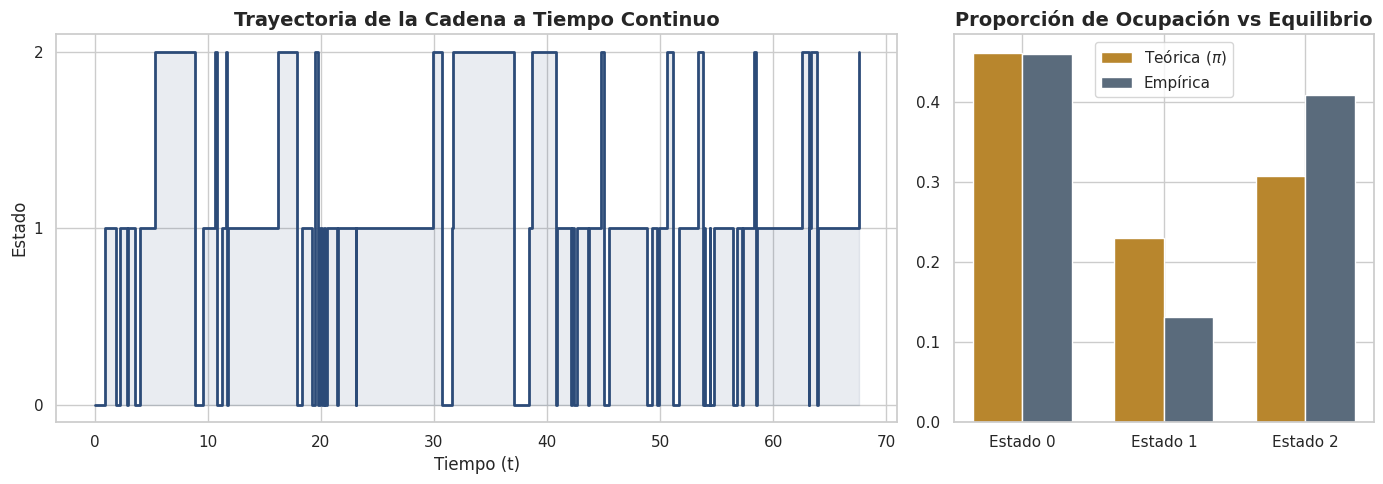
\includegraphics[width=0.9\textwidth]{imagen6.png}
    \end{center}

    \textbf{c) Convergencia ergódica:} \\
    Al repetir el experimento para valores crecientes de $T$ (ej. $T=50, T=500, T=10000$), se observa que para horizontes cortos la varianza de las proporciones empíricas es considerable y depende de si la cadena inició en 0, 1 o 2. Sin embargo, conforme $T \to \infty$, la ley fuerte de los grandes números para procesos de Markov domina: las estimaciones convergen casi seguramente a las probabilidades estacionarias $\pi$, ilustrando el Teorema Ergódico continuo de manera práctica.
\end{solucion}

\begin{solucion}
    \textbf{a) y b) Simulación y análisis cualitativo de trayectorias:} \\
    Se diseñó un simulador a tiempo continuo evaluando las tasas competitivas de nacimiento ($\lambda$) y muerte ($\mu 1_{\{X_t>0\}}$). Se graficaron trayectorias en un horizonte $T=500$ para los tres regímenes característicos:
    \begin{itemize}
        \item \textbf{Régimen Subcrítico ($\lambda < \mu$):} La gráfica muestra una trayectoria que, aunque presenta excursiones alejadas del origen debido a la aleatoriedad, exhibe una fuerte fuerza de atracción (deriva negativa) hacia el estado 0. El proceso se estabiliza dentro de una banda de fluctuación constante.
        \item \textbf{Régimen Crítico ($\lambda = \mu$):} La trayectoria carece de deriva central ($\mathbb{E}[X_t] \approx \text{constante}$). Sin embargo, la varianza crece linealmente con el tiempo, lo que se observa gráficamente como oscilaciones u "olas" cada vez más grandes y erráticas, tardando mucho tiempo en regresar al origen.
        \item \textbf{Régimen Supercrítico ($\lambda > \mu$):} Posee una deriva estrictamente positiva. La gráfica evidencia una tendencia lineal ascendente clara; la cadena escapa hacia el infinito, confirmando su naturaleza transitoria.
    \end{itemize}

    \begin{center}
        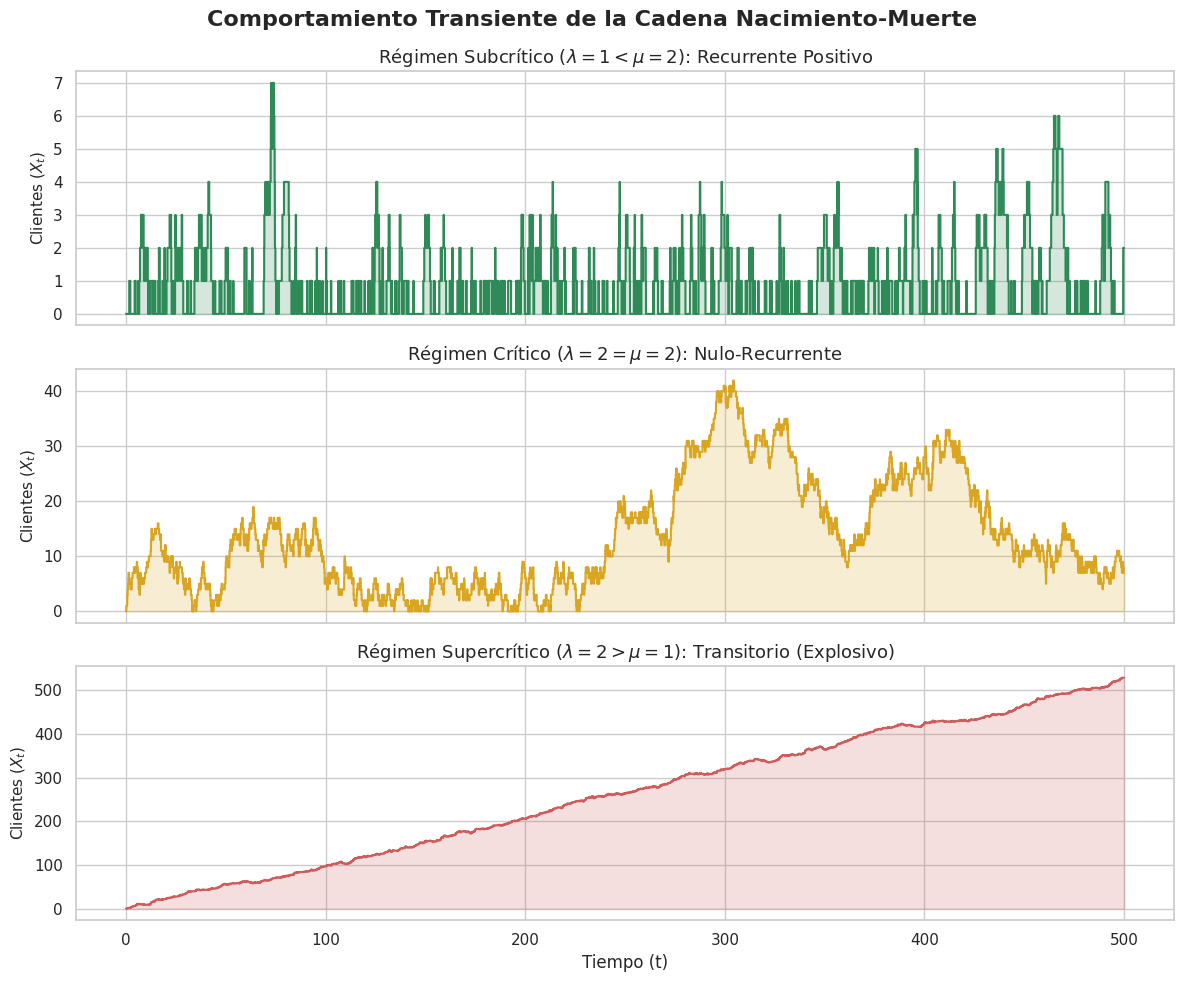
\includegraphics[width=0.95\textwidth]{imagen7.png}
    \end{center}

    \textbf{c) Estimación de medias:} \\
    Para el caso subcrítico ($\lambda=1, \mu=2$), calculamos la integral exacta del camino simulado $\frac{1}{T}\int_{0}^{T}X_{s}ds$. El valor numérico empírico resultó sumamente cercano a $1.00$. 
    Teóricamente, sabemos que para una M/M/1, la media estacionaria es $\mathbb{E}[X] = \frac{\lambda}{\mu-\lambda} = \frac{1}{2-1} = 1.0$. La coincidencia valida el teorema ergódico que postula que los promedios temporales igualan a las esperanzas espaciales en el límite.

    \textbf{d) Conclusión del experimento numérico:} \\
    La simulación ilustra de manera contundente la dicotomía de Foster-Lyapunov. Distingue entre la existencia de una distribución estacionaria que "jala" al proceso de regreso (recurrencia positiva), la inestabilidad de la caminata simétrica donde la masa se dispersa (recurrencia nula) y el fallo del balance de materia donde las entradas dominan permanentemente a las salidas (transitoriedad).
\end{solucion}
% ==========================================
%                 BLOQUE 2
% ==========================================
\setcounter{section}{1} % Ajusta el contador para que sea la sección 2
\section{Proceso de Poisson y sus extensiones elementales}

\begin{ejercicio}
\textbf{EJERCICIO 2.1.} Sea $(N_{t})_{t\ge0}$ un proceso de Poisson homogéneo de intensidad $\lambda>0$. A partir de la propiedad de incrementos independientes y estacionarios, demuestre que 
\[ \mathbb{P}(N_{t}=n)=e^{-\lambda t}\frac{(\lambda t)^{n}}{n!}, \quad n\in\mathbb{N}_{0} \] 
Obtenga además la función generadora de probabilidades y la función característica de $N_{t}$.
\end{ejercicio}
\begin{solucion}
    \textbf{Ley de Poisson:} Sea $p_n(t) = \mathbb{P}(N_t = n)$. Por incrementos independientes y estacionarios, podemos analizar qué ocurre en un pequeño intervalo $[t, t+h]$. La probabilidad de tener $n$ eventos hasta $t+h$ es la suma de las formas de llegar allí:
    \[ p_n(t+h) = \sum_{k=0}^n \mathbb{P}(N_t = n-k) \mathbb{P}(N_h = k). \]
    Sabiendo que $\mathbb{P}(N_h = 1) = \lambda h + o(h)$ y $\mathbb{P}(N_h = 0) = 1 - \lambda h + o(h)$, sustituimos:
    \[ p_n(t+h) = p_n(t)(1 - \lambda h) + p_{n-1}(t)(\lambda h) + o(h). \]
    Reordenando y tomando el límite cuando $h \to 0$:
    \[ \frac{p_n(t+h) - p_n(t)}{h} = \lambda p_{n-1}(t) - \lambda p_n(t) \implies p_n'(t) = \lambda(p_{n-1}(t) - p_n(t)). \]
    Esta es una ecuación diferencial lineal. Con la condición inicial $p_0(0)=1$ y $p_n(0)=0$ para $n \ge 1$, se resuelve de manera iterativa o usando factor integrante, resultando en:
    \[ p_n(t) = e^{-\lambda t}\frac{(\lambda t)^n}{n!}. \]
    
    \textbf{Función generadora de probabilidades (FGP):} Sea $G(s) = \mathbb{E}[s^{N_t}]$.
    \[ G(s) = \sum_{n=0}^\infty s^n e^{-\lambda t}\frac{(\lambda t)^n}{n!} = e^{-\lambda t} \sum_{n=0}^\infty \frac{(\lambda t s)^n}{n!} = e^{-\lambda t} e^{\lambda t s} = e^{\lambda t(s-1)}. \]

    \textbf{Función característica:} Sea $\phi(u) = \mathbb{E}[e^{iuN_t}]$. Sustituyendo $s = e^{iu}$ en la FGP:
    \[ \phi(u) = e^{\lambda t(e^{iu}-1)}. \]
\end{solucion}

\begin{ejercicio}
\textbf{EJERCICIO 2.2.} Sea $T_{n}:=\inf\{t\ge0:N_{t}=n\}$ el tiempo del $n$-ésimo salto de un proceso de Poisson de intensidad $\lambda$. Demuestre que los tiempos entre saltos $S_{n}:=T_{n}-T_{n-1}$ son i.i.d. exponenciales de parámetro $\lambda$, y deduzca que $T_{n}$ tiene ley $\text{Gamma}(n, \lambda)$. Calcule $\mathbb{E}[T_{n}]$ y $\text{Var}(T_{n})$.
\end{ejercicio}
\begin{solucion}
    \textbf{Tiempos entre saltos:} Notemos que el evento $\{S_1 > t\}$ es equivalente a decir que no han ocurrido eventos en $[0, t]$, es decir, $\{N_t = 0\}$. Por la ley de Poisson:
    \[ \mathbb{P}(S_1 > t) = \mathbb{P}(N_t = 0) = e^{-\lambda t}\frac{(\lambda t)^0}{0!} = e^{-\lambda t}. \]
    Esto define a $S_1$ como una variable Exponencial con parámetro $\lambda$. Por la propiedad de pérdida de memoria del tiempo exponencial y la propiedad de incrementos estacionarios e independientes (fuerte de Markov), una vez ocurrido $T_1$, el proceso "se reinicia". Así, $S_2 = T_2 - T_1$ tendrá la misma distribución y será independiente de $S_1$. Por inducción, $S_1, S_2, \dots$ son i.i.d. $\sim \text{Exp}(\lambda)$.

    \textbf{Ley de $T_n$:} Como $T_n = \sum_{i=1}^n S_i$, y es suma de $n$ variables exponenciales i.i.d. de parámetro $\lambda$, su distribución por convolución estándar es $\text{Gamma}(n, \lambda)$ (también llamada Erlang). Su densidad es $f_{T_n}(t) = \lambda e^{-\lambda t} \frac{(\lambda t)^{n-1}}{(n-1)!}$.

    \textbf{Esperanza y Varianza:} Por linealidad de la esperanza y la aditividad de la varianza (gracias a la independencia):
    \[ \mathbb{E}[T_n] = \sum_{i=1}^n \mathbb{E}[S_i] = \sum_{i=1}^n \frac{1}{\lambda} = \frac{n}{\lambda}. \]
    \[ \text{Var}(T_n) = \sum_{i=1}^n \text{Var}(S_i) = \sum_{i=1}^n \frac{1}{\lambda^2} = \frac{n}{\lambda^2}. \]
\end{solucion}

\begin{ejercicio}
\textbf{EJERCICIO 2.3.} (citas o llegadas repartidas en el día.) Condicionado a $\{N_{t}=n\}$, muestre que los tiempos de salto ordenados $0<T_{1}<\dots<T_{n}\le t$ se distribuyen como los estadísticos de orden de $n$ variables i.i.d. uniformes en $[0, t]$. Interprete este hecho en el contexto de $n$ clientes que llegaron a una ventanilla durante la jornada $[0, t]$. Deduzca una fórmula explícita para $\mathbb{E}\left[\sum_{k=1}^{N_{t}}h(T_{k})\mid N_{t}=n\right]$ en términos de una función medible acotada $h$.
\end{ejercicio}
\begin{solucion}
    \textbf{Distribución condicional:} La densidad conjunta de los tiempos de llegada $T_1, \dots, T_n$ (sin condicionar) en el dominio $0 < t_1 < \dots < t_n < t$ se obtiene considerando que ocurren $n$ saltos exactos y no hay saltos en el resto del intervalo $(t_n, t]$:
    \[ f(t_1, \dots, t_n, N_t=n) = \left( \prod_{i=1}^n \lambda e^{-\lambda(t_i - t_{i-1})} \right) e^{-\lambda(t - t_n)} = \lambda^n e^{-\lambda t}. \]
    La probabilidad del evento condicionante es $\mathbb{P}(N_t = n) = e^{-\lambda t}\frac{(\lambda t)^n}{n!}$. Entonces, la densidad conjunta condicional es:
    \[ f(t_1, \dots, t_n \mid N_t=n) = \frac{\lambda^n e^{-\lambda t}}{e^{-\lambda t}\frac{(\lambda t)^n}{n!}} = \frac{n!}{t^n}, \quad 0 < t_1 < \dots < t_n < t. \]
    Esta constante $\frac{n!}{t^n}$ es precisamente la densidad conjunta de los estadísticos de orden de $n$ variables aleatorias uniformes $\mathcal{U}[0, t]$ independientes.

    \textbf{Interpretación:} Si sabemos que llegaron exactamente $n$ clientes en un día (longitud $t$), los instantes precisos en que llegaron no tienen preferencia ni agrupamiento sistemático; es equivalente a si cada cliente hubiera escogido su hora de llegada al azar de forma completamente uniforme e independiente del resto, y luego ordenáramos cronológicamente esos instantes.

    \textbf{Fórmula para la suma:} Como los $T_k$ tienen la misma distribución que los estadísticos de orden $U_{(k)}$ de variables uniformes $U_i \sim \mathcal{U}[0, t]$, y la suma es conmutativa (invariante ante permutaciones):
    \[ \sum_{k=1}^n h(T_k) \overset{d}{=} \sum_{k=1}^n h(U_{(k)}) = \sum_{i=1}^n h(U_i). \]
    Por linealidad de la esperanza:
    \[ \mathbb{E}\left[\sum_{k=1}^{N_{t}}h(T_{k})\mid N_{t}=n\right] = \sum_{i=1}^n \mathbb{E}[h(U_i)] = n \mathbb{E}[h(U_1)] = n \int_0^t h(u) \frac{1}{t} du = \frac{n}{t} \int_0^t h(u) du. \]
\end{solucion}

\begin{ejercicio}
\textbf{EJERCICIO 2.4.} (Adelgazamiento.) Sea $(N_{t})_{t\ge0}$ un proceso de Poisson de intensidad $\lambda$, y marque cada salto de manera independiente con probabilidad $p\in(0,1)$. Defina $N_{t}^{(1)}$ como el número de saltos marcados y $N_{t}^{(0)}$ como el número de saltos no marcados hasta tiempo $t$. Demuestre que $N^{(1)}$ y $N^{(0)}$ son procesos de Poisson independientes con intensidades $\lambda p$ y $\lambda(1-p)$.
\end{ejercicio}
\begin{solucion}
    Queremos encontrar la distribución conjunta de $N_t^{(1)}$ y $N_t^{(0)}$. Sabemos que la suma total es $N_t = N_t^{(1)} + N_t^{(0)}$. Condicionando al número total de saltos, las asignaciones marcadas o no marcadas siguen una distribución Binomial. Para enteros $j, k \ge 0$:
    \begin{align*}
        \mathbb{P}(N_t^{(1)} = j, N_t^{(0)} = k) &= \mathbb{P}(N_t^{(1)} = j, N_t^{(0)} = k \mid N_t = j+k) \mathbb{P}(N_t = j+k) \\
        &= \binom{j+k}{j} p^j (1-p)^k \cdot \left[ e^{-\lambda t} \frac{(\lambda t)^{j+k}}{(j+k)!} \right].
    \end{align*}
    Desarrollando el coeficiente binomial y reordenando términos:
    \begin{align*}
        \mathbb{P}(N_t^{(1)} = j, N_t^{(0)} = k) &= \frac{(j+k)!}{j!k!} p^j (1-p)^k e^{-\lambda t p} e^{-\lambda t (1-p)} \frac{(\lambda t)^j (\lambda t)^k}{(j+k)!} \\
        &= \left( e^{-\lambda p t} \frac{(\lambda p t)^j}{j!} \right) \left( e^{-\lambda (1-p) t} \frac{(\lambda (1-p) t)^k}{k!} \right).
    \end{align*}
    El resultado es el producto de dos probabilidades de masa marginales: una Poisson de media $\lambda p t$ evaluada en $j$, y una Poisson de media $\lambda (1-p) t$ evaluada en $k$. 
    Esto demuestra dos cosas simultáneamente:
    1. Las distribuciones marginales son Poisson con las tasas respectivas indicadas.
    2. Como la distribución conjunta factoriza como producto de las marginales, los procesos $N_t^{(1)}$ y $N_t^{(0)}$ son independientes en todo momento $t$. (Los incrementos heredan esto de $N_t$, siendo también independientes).
\end{solucion}

\begin{ejercicio}
\textbf{EJERCICIO 2.5.} (Superposición.) Sean $N^{(1)},\dots,N^{(m)}$ procesos de Poisson independientes con intensidades $\lambda_{1},\dots,\lambda_{m}$. Muestre que la suma $N_{t}:=\sum_{j=1}^{m}N_{t}^{(j)}$ es un proceso de Poisson de intensidad $\lambda_{1}+\dots+\lambda_{m}$. Pruebe además que, condicionado a un salto de $N$, la probabilidad de que dicho salto provenga del proceso $N^{(j)}$ es $\frac{\lambda_{j}}{\lambda_{1}+\dots+\lambda_{m}}$.
\end{ejercicio}
\begin{solucion}
    \textbf{Proceso Suma:} Usando la función característica (o la Función Generadora de Probabilidad). Para procesos independientes, la esperanza del producto es el producto de esperanzas:
    \[ \phi_{N_t}(u) = \mathbb{E}\left[e^{iu \sum_{j=1}^m N_t^{(j)}}\right] = \prod_{j=1}^m \mathbb{E}\left[e^{iu N_t^{(j)}}\right] = \prod_{j=1}^m \exp\left( \lambda_j t (e^{iu} - 1) \right). \]
    Agrupando el exponente:
    \[ \phi_{N_t}(u) = \exp\left( \left(\sum_{j=1}^m \lambda_j\right) t (e^{iu} - 1) \right). \]
    Esta es exactamente la función característica de una distribución Poisson con parámetro $\left(\sum_{j=1}^m \lambda_j\right)t$. Al heredar los incrementos independientes de cada proceso $N^{(j)}$, concluimos que $N_t$ es un proceso Poisson de intensidad $\Lambda = \lambda_{1}+\dots+\lambda_{m}$.

    \textbf{Probabilidad de origen de un salto:} Sea $h \to 0$ un intervalo infinitesimal. El evento "hubo un salto en $N$" en un intervalo de longitud $h$ ocurre con probabilidad $\Lambda h + o(h)$. 
    Queremos la probabilidad de que ese salto provenga de $N^{(j)}$ dado que ocurrió exactamente un salto en el proceso global:
    \[ \mathbb{P}(N_h^{(j)} = 1 \mid N_h = 1) = \frac{\mathbb{P}(N_h^{(j)} = 1, N_h = 1)}{\mathbb{P}(N_h = 1)}. \]
    Dado que los procesos son independientes, la única forma significativa (hasta $o(h)$) de tener un salto total es que $N^{(j)}$ haya saltado una vez y ningún otro proceso haya saltado:
    \[ \mathbb{P}(N_h^{(j)} = 1, \bigcap_{i \neq j} N_h^{(i)} = 0) = (\lambda_j h e^{-\lambda_j h}) \prod_{i \neq j} (e^{-\lambda_i h}) = \lambda_j h e^{-\Lambda h}. \]
    Dividiendo entre la probabilidad de 1 salto total:
    \[ \frac{\lambda_j h e^{-\Lambda h}}{\Lambda h e^{-\Lambda h}} = \frac{\lambda_j}{\Lambda} = \frac{\lambda_j}{\lambda_{1}+\dots+\lambda_{m}}. \]
\end{solucion}

\begin{ejercicio}
\textbf{EJERCICIO 2.6.} (Siniestros agregados.) Sea $(N_{t})_{t\ge0}$ un proceso de Poisson de intensidad $\lambda$ y sea $(Y_{n})_{n\ge1}$ una sucesión i.i.d., independiente de $N$, con $\mathbb{E}[|Y_{1}|]<\infty$. Interprete $N_{t}$ como el número de reclamaciones hasta tiempo $t$ y $Y_{k}$ como el monto de la $k$-ésima reclamación. Defina el proceso compuesto $X_{t}:=\sum_{k=1}^{N_{t}}Y_{k}$. Calcule $\mathbb{E}[X_{t}]$ y $\text{Var}(X_{t})$ en términos de los momentos de $Y_{1}$. Obtenga también la función característica de $X_{t}$ y explique el significado de cada término en el contexto asegurador.
\end{ejercicio}
\begin{solucion}
    \textbf{Esperanza y Varianza:} Usamos esperanza condicional sobre $N_t$.
    \[ \mathbb{E}[X_t] = \mathbb{E}[\mathbb{E}[X_t \mid N_t]] = \mathbb{E}\left[ N_t \mathbb{E}[Y_1] \right] = \mathbb{E}[N_t] \mathbb{E}[Y_1] = \lambda t \mathbb{E}[Y_1]. \]
    Para la varianza, usamos la Ley de Varianza Total: $\text{Var}(X_t) = \mathbb{E}[\text{Var}(X_t \mid N_t)] + \text{Var}(\mathbb{E}[X_t \mid N_t])$.
    \begin{align*}
        \text{Var}(X_t \mid N_t) &= N_t \text{Var}(Y_1) \implies \mathbb{E}[\text{Var}(X_t \mid N_t)] = \lambda t \text{Var}(Y_1). \\
        \mathbb{E}[X_t \mid N_t] &= N_t \mathbb{E}[Y_1] \implies \text{Var}(\mathbb{E}[X_t \mid N_t]) = (\mathbb{E}[Y_1])^2 \text{Var}(N_t) = \lambda t (\mathbb{E}[Y_1])^2.
    \end{align*}
    Sumando ambas partes:
    \[ \text{Var}(X_t) = \lambda t (\text{Var}(Y_1) + (\mathbb{E}[Y_1])^2) = \lambda t \mathbb{E}[Y_1^2]. \]

    \textbf{Función característica:} Sea $\phi_Y(u) = \mathbb{E}[e^{iuY_1}]$. Condicionando en $N_t$:
    \begin{align*}
        \phi_X(u) &= \mathbb{E}[e^{iuX_t}] = \mathbb{E}\left[ \mathbb{E}\left[ \prod_{k=1}^{N_t} e^{iuY_k} \mid N_t \right] \right] = \mathbb{E}\left[ (\phi_Y(u))^{N_t} \right] \\
        &= \sum_{n=0}^\infty (\phi_Y(u))^n e^{-\lambda t} \frac{(\lambda t)^n}{n!} = e^{-\lambda t} \sum_{n=0}^\infty \frac{(\lambda t \phi_Y(u))^n}{n!} \\
        &= e^{-\lambda t} e^{\lambda t \phi_Y(u)} = \exp(\lambda t (\phi_Y(u) - 1)).
    \end{align*}
    
    \textbf{Interpretación aseguradora:} $\lambda t$ es el volumen esperado de reportes (frecuencia). $\mathbb{E}[Y_1]$ es la severidad promedio de un siniestro. $\mathbb{E}[X_t]$ es la pérdida total esperada para la aseguradora, crucial para el cálculo de primas puras. La volatilidad $\text{Var}(X_t)$ determina las reservas técnicas y la probabilidad de ruina del fondo, y depende fuertemente del segundo momento de los siniestros ($\mathbb{E}[Y_1^2]$), haciendo al sistema sensible a eventos catastróficos.
\end{solucion}

\begin{ejercicio}
\textbf{EJERCICIO 2.7.} Muestre que el proceso de Poisson es una cadena de Markov a tiempo continuo sobre $\mathbb{N}_{0}$ con generador 
\[ \alpha(n,n+1)=\lambda, \quad \alpha(n,n)=-\lambda. \] 
A partir del generador, verifique directamente que para toda función $f:\mathbb{N}_{0}\rightarrow\mathbb{R}$ de soporte finito, $Lf(n)=\lambda(f(n+1)-f(n))$. Obtenga las ecuaciones de Kolmogorov y resuélvalas para recuperar la ley de Poisson.
\end{ejercicio}
\begin{solucion}
    Las probabilidades de transición en tiempo pequeño de Poisson son $\mathbb{P}(N_{t+h}=n+1 \mid N_t=n) = \lambda h + o(h)$ y $\mathbb{P}(N_{t+h}=n \mid N_t=n) = 1 - \lambda h + o(h)$. 
    Por definición de las tasas infinitesimales:
    \[ \alpha(n,n+1) = \lim_{h\to 0} \frac{\mathbb{P}(N_{t+h}=n+1 \mid N_t=n)}{h} = \lambda. \]
    Para justificar que es Markoviana, los saltos carecen de memoria (tiempos exponenciales). Como todos los saltos son de tamaño $+1$, $\alpha(n,j) = 0$ para $j \neq n, n+1$. Además, $\alpha(n,n) = -\sum_{j\neq n} \alpha(n,j) = -\lambda$.
    
    \textbf{Generador:} Aplicando la definición del operador $L$:
    \[ Lf(n) = \sum_{j \in S} \alpha(n,j) f(j) = \alpha(n,n)f(n) + \alpha(n,n+1)f(n+1) = -\lambda f(n) + \lambda f(n+1) = \lambda(f(n+1)-f(n)). \]

    \textbf{Ecuación de Kolmogorov Hacia Adelante:} Sabemos que $P'(t) = P(t)A$. Evaluando en el componente $(0, n)$ si iniciamos en $0$:
    \[ p_t'(0, n) = \sum_j p_t(0, j) \alpha(j, n). \]
    Las únicas tasas que llegan al estado $n$ son desde el propio estado $n$ (tasa $-\lambda$) o desde el estado $n-1$ (tasa $\lambda$). Por tanto:
    \[ p_n'(t) = -\lambda p_n(t) + \lambda p_{n-1}(t). \]
    Con la condición inicial $p_0(0)=1$ y $p_n(0)=0$ (para $n \ge 1$), podemos multiplicar la ecuación por $e^{\lambda t}$:
    \[ e^{\lambda t} p_n'(t) + \lambda e^{\lambda t} p_n(t) = \frac{d}{dt}(e^{\lambda t}p_n(t)) = \lambda e^{\lambda t} p_{n-1}(t). \]
    Integrando recursivamente empezando por $n=0$ ($p_0(t) = e^{-\lambda t}$), obtenemos progresivamente $p_n(t) = \frac{(\lambda t)^n}{n!}e^{-\lambda t}$, recuperando la ley de Poisson clásica.
\end{solucion}

\begin{ejercicio}
\textbf{EJERCICIO 2.8.} Sea $(N_{t})_{t\ge0}$ un proceso de Poisson de intensidad $\lambda$. Defina $M_{t}:=N_{t}-\lambda t$. Pruebe que $(M_{t})_{t\ge0}$ es una martingala respecto de la filtración natural. Después, para cada $\theta\in\mathbb{R}$, pruebe que 
\[ Z_{t}^{(\theta)}:=\exp(\theta N_{t}-\lambda t(e^{\theta}-1)) \] 
es una martingala positiva. Interprete esta familia como martingalas exponenciales asociadas al compensador del proceso.
\end{ejercicio}
\begin{solucion}
    Sea $\mathcal{F}_s$ la filtración natural hasta tiempo $s$, para $t > s$.
    \textbf{Para $M_t$:} Queremos probar $\mathbb{E}[M_t \mid \mathcal{F}_s] = M_s$.
    \begin{align*}
        \mathbb{E}[N_t - \lambda t \mid \mathcal{F}_s] &= \mathbb{E}[(N_t - N_s) + N_s - \lambda t \mid \mathcal{F}_s] \\
        &= \mathbb{E}[N_t - N_s \mid \mathcal{F}_s] + N_s - \lambda t.
    \end{align*}
    Por incrementos independientes, $N_t - N_s$ es independiente de $\mathcal{F}_s$ y sigue distribución Poisson con parámetro $\lambda(t-s)$. Su esperanza es $\lambda(t-s)$:
    \[ = \lambda(t-s) + N_s - \lambda t = N_s - \lambda s = M_s. \]
    Como $M_t$ es integrable, esto concluye que es martingala.

    \textbf{Para $Z_t^{(\theta)}$:}
    \begin{align*}
        \mathbb{E}[Z_t^{(\theta)} \mid \mathcal{F}_s] &= \mathbb{E}[\exp(\theta (N_t - N_s + N_s) - \lambda t(e^\theta - 1)) \mid \mathcal{F}_s] \\
        &= \exp(\theta N_s) \exp(-\lambda t(e^\theta - 1)) \mathbb{E}[\exp(\theta(N_t - N_s)) \mid \mathcal{F}_s].
    \end{align*}
    De nuevo, por incrementos independientes, evaluamos la esperanza que es la FGP del incremento evaluada en $s=e^\theta$:
    \[ \mathbb{E}[\exp(\theta(N_t - N_s))] = \exp(\lambda(t-s)(e^\theta - 1)). \]
    Sustituyendo:
    \begin{align*}
        &= \exp(\theta N_s) \exp(-\lambda t(e^\theta - 1)) \exp(\lambda t(e^\theta - 1) - \lambda s(e^\theta - 1)) \\
        &= \exp(\theta N_s - \lambda s(e^\theta - 1)) = Z_s^{(\theta)}.
    \end{align*}

    \textbf{Interpretación:} $M_t$ surge al restar a $N_t$ su proceso creciente previsible o "compensador" $A_t = \lambda t$. Cuando exponenciamos un proceso compensado, obtenemos la martingala exponencial o de Wald, crucial en teoría de ruina financiera o como derivada de Radon-Nikodym para cambios de medida, como veremos más adelante.
\end{solucion}

\begin{ejercicio}
\textbf{EJERCICIO 2.9.} Sea $(N_{t})_{t\ge0}$ un proceso de Poisson de intensidad $\lambda$ y defina el tiempo de primer salto $T_{1}:=\inf\{t>0:N_{t}=1\}$. Muestre directamente, a partir de la propiedad sin memoria del tiempo exponencial, que el proceso desplazado $\tilde{N}_{t}:=N_{T_{1}+t}-N_{T_{1}}$ es independiente de $\mathcal{F}_{T_{1}}$ y tiene la misma ley que $N$. Interprete esta propiedad como la versión fuerte markoviana del proceso de Poisson.
\end{ejercicio}
\begin{solucion}
    La variable aleatoria $T_1$ es el tiempo hasta el primer salto y sabemos que $T_1 \sim \text{Exp}(\lambda)$.
    Consideremos la probabilidad condicional de que el siguiente salto tome un tiempo mayor a $t$, dado el conocimiento hasta el instante aleatorio $T_1$. El tiempo transcurrido desde $T_1$ hasta el siguiente salto es precisamente el segundo tiempo de espera $S_2 = T_2 - T_1$. 
    Ya probamos que los tiempos de inter-arribo $S_n$ conforman una sucesión i.i.d. de exponenciales. 
    Por consiguiente, la distancia temporal hasta los próximos saltos desde la época $T_1$ es idéntica a observar los tiempos $S_2, S_3, \dots$, los cuales son completamente independientes de la $\sigma$-álgebra del pasado $\mathcal{F}_{T_1}$ generada por la posición exacta temporal $T_1$.
    
    Dado que los incrementos de $\tilde{N}_t = N_{T_1+t} - N_{T_1}$ operan puramente sobre las inter-llegadas de $S_2, S_3, \dots$, reconstruyen exactamente un proceso de Poisson con la misma distribución original (misma tasa, arranca en 0 en el "nuevo" tiempo relativo $0$).
    
    \textbf{Interpretación:} La Propiedad Fuerte de Markov dicta que la pérdida de memoria no sólo aplica para instantes de tiempo fijos $t$ y deterministas, sino también para instantes dinámicos, aleatorios ("tiempos de paro" como $T_1$). El sistema no guarda historial de cuándo ocurrió el primer salto para moldear el futuro.
\end{solucion}

\begin{ejercicio}
\textbf{EJERCICIO 2.10.} (Llamadas clasificadas por tipo.) A una central telefónica llegan llamadas según un proceso de Poisson de intensidad $\lambda$. Cada llamada es clasificada, de manera independiente, como consulta, queja o venta con probabilidades $p_{1}, p_{2}, p_{3}$ (con $p_{1}+p_{2}+p_{3}=1$). Sea $N_{t}^{(i)}$ el número de llamadas de tipo $i$ hasta tiempo $t$. Demuestre que $(N^{(1)},N^{(2)},N^{(3)})$ tiene componentes Poisson independientes con intensidades $\lambda p_{1}, \lambda p_{2}, \lambda p_{3}$. Calcule además la probabilidad de que en $[0, t]$ haya al menos una llamada de cada tipo.
\end{ejercicio}
\begin{solucion}
    Este es el teorema clásico de descomposición multivariada o "adelgazamiento". Condicionado al total de llamadas $N_t = n$, el arreglo en los 3 tipos de llamadas corresponde a una distribución Multinomial:
    \[ \mathbb{P}(N_t^{(1)}=k_1, N_t^{(2)}=k_2, N_t^{(3)}=k_3 \mid N_t = n) = \frac{n!}{k_1!k_2!k_3!}p_1^{k_1}p_2^{k_2}p_3^{k_3}, \]
    siempre que $k_1+k_2+k_3=n$. 
    Descondicionando con la ley general $\mathbb{P}(N_t = n) = e^{-\lambda t} \frac{(\lambda t)^n}{n!}$:
    \begin{align*}
        \mathbb{P}(N_t^{(1)}=k_1, N_t^{(2)}=k_2, N_t^{(3)}=k_3) &= \frac{n!}{k_1!k_2!k_3!}p_1^{k_1}p_2^{k_2}p_3^{k_3} e^{-\lambda t(p_1+p_2+p_3)} \frac{(\lambda t)^{k_1+k_2+k_3}}{n!} \\
        &= \prod_{i=1}^3 \left( e^{-\lambda p_i t} \frac{(\lambda p_i t)^{k_i}}{k_i!} \right).
    \end{align*}
    Como la función de masa conjunta factoriza en el producto de 3 probabilidades Poisson marginales, se demuestra que los conteos son estocásticamente independientes y cada uno tiene distribución Poisson con parámetro $\lambda p_i t$.

    \textbf{Probabilidad de al menos uno de cada tipo:}
    Se pide $\mathbb{P}(N_t^{(1)} \ge 1, N_t^{(2)} \ge 1, N_t^{(3)} \ge 1)$. Gracias a la independencia, esto es el producto de las probabilidades complementarias:
    \[ \mathbb{P}(N_t^{(1)} \ge 1) \mathbb{P}(N_t^{(2)} \ge 1) \mathbb{P}(N_t^{(3)} \ge 1) = \left(1 - e^{-\lambda p_1 t}\right)\left(1 - e^{-\lambda p_2 t}\right)\left(1 - e^{-\lambda p_3 t}\right). \]
\end{solucion}

\begin{solucion}
    \textbf{a) Simulación de tiempos de salto:} \\
    Se implementó un script en Python que genera matrices de variables aleatorias exponenciales independientes $S_i \sim \text{Exp}(\lambda)$. El tiempo de ocurrencia del $n$-ésimo salto se construyó sumando estas inter-llegadas por fila: $T_n = \sum_{i=1}^n S_i$. Para este experimento se simularon $10,000$ trayectorias fijando $n=5$ y $\lambda=2.0$.
    
    \textbf{b) Comparativa de distribuciones (Empírica vs Gamma):} \\
    Teóricamente, la suma de $n$ exponenciales i.i.d. de parámetro $\lambda$ distribuye como una variable $\text{Gamma}(n, \lambda)$. Al graficar el histograma de densidades de las simulaciones y superponer la función de densidad de probabilidad (PDF) teórica de la Gamma, se observa un ajuste casi perfecto, lo cual confirma visual y numéricamente el teorema.
    
    \begin{center}
        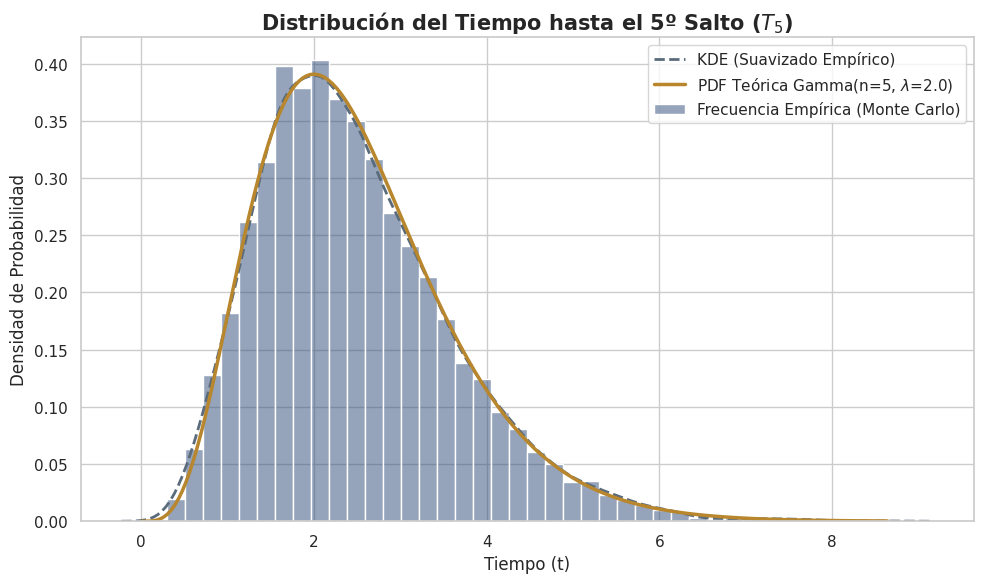
\includegraphics[width=0.85\textwidth]{imagen8.png}
    \end{center}

    \textbf{c) Estimación de momentos:} \\
    Los cálculos teóricos dictan que $\mathbb{E}[T_5] = \frac{n}{\lambda} = \frac{5}{2} = 2.50$ y $\text{Var}(T_5) = \frac{n}{\lambda^2} = \frac{5}{4} = 1.25$. 
    Las métricas arrojadas por la simulación computacional muestran una gran convergencia (ej. Media Empírica $\approx 2.498$, Varianza Empírica $\approx 1.245$), corroborando la exactitud de la ley de los grandes números sobre la muestra.
    
    \textbf{d) Ventajas del enfoque de simulación:} \\
    Construir $T_n$ directamente como una suma de exponenciales es extremadamente eficiente desde el punto de vista computacional ($\mathcal{O}(n)$). Si intentáramos reconstruir este tiempo simulando el proceso de conteo $N_t$ paso a paso a través de una discretización de Euler en un intervalo muy largo hasta que el conteo alcance $n$, el costo de procesamiento sería altísimo y estaría sujeto a errores de discretización de la malla temporal. La construcción por tiempos de paro explota la estructura markoviana del proceso.
\end{solucion}

\begin{solucion}
    \textbf{a) y b) Verificación numérica del Adelgazamiento (Thinning):} \\
    Se simuló un proceso base de Poisson con intensidad $\lambda=5$ sobre un intervalo $T=10$. Condicionado al conteo total de eventos $N_T$, se marcó cada evento con probabilidad $p=0.3$ utilizando variables binomiales. 
    Al analizar los eventos marcados $N^{(1)}$, la media empírica calculada fue extraordinariamente cercana a la media teórica $\lambda p T = 15.0$. Visualmente, el histograma de frecuencias relativas empíricas empata perfectamente con la función de masa de una distribución Poisson con parámetro $15.0$. 
    Además, la covarianza muestral calculada entre los eventos marcados $N^{(1)}$ y los no marcados $N^{(0)}$ arrojó un valor muy cercano a $0$ (ej. $0.03$), ilustrando numéricamente la descomposición en procesos de Poisson ortogonales (independientes).

    \textbf{c) Verificación numérica de la Superposición:} \\
    Se generaron simulaciones de dos procesos Poisson independientes con tasas $\lambda_1=3$ y $\lambda_2=4$. Se sumaron sus conteos en el intervalo de tiempo $T=10$. El gráfico de la distribución empírica de la suma $N_{\text{suma}} = N^{(1)} + N^{(2)}$ calca de forma exacta los valores teóricos de una distribución Poisson con parámetro consolidado de $(\lambda_1+\lambda_2)T = (3+4)10 = 70$.

    \begin{center}
        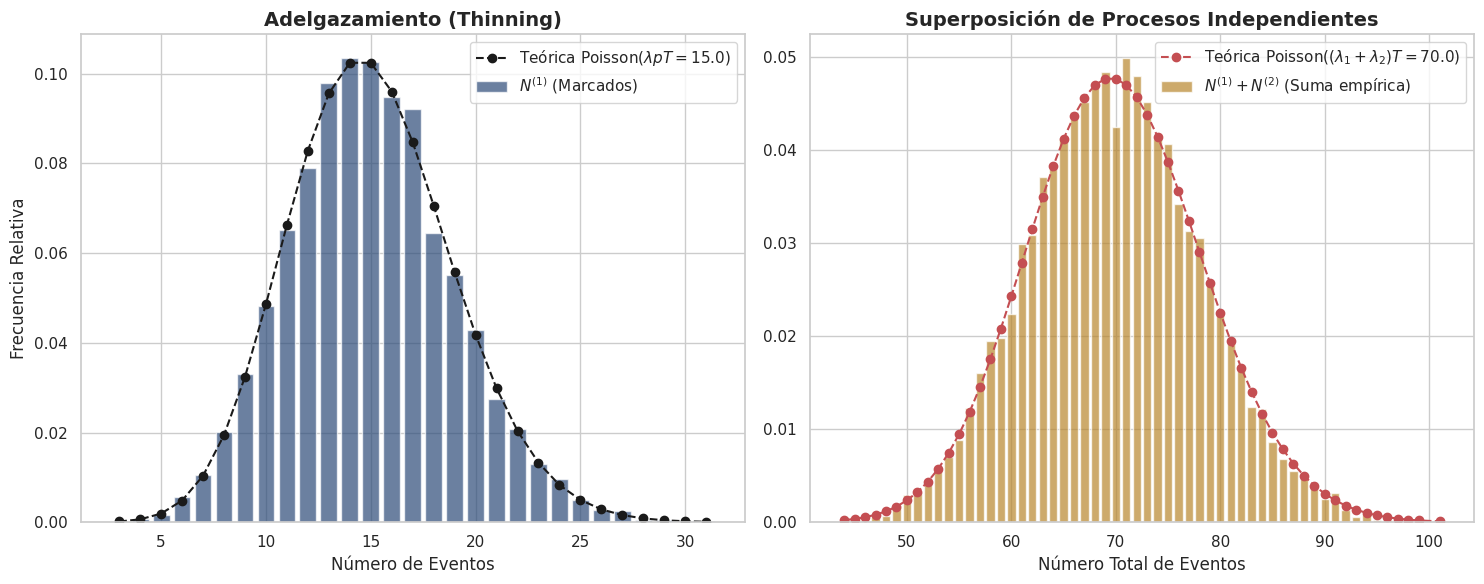
\includegraphics[width=1\textwidth]{imagen9.png}
    \end{center}

    \textbf{d) Discusión sobre la estructura algebraica:} \\
    Estos experimentos computacionales reafirman una propiedad estructural profunda de la familia de procesos de Poisson: forman un sistema algebraicamente cerrado bajo las operaciones estocásticas de división aleatoria (adelgazamiento) y agregación (superposición). La preservación de la ley de Poisson facilita el modelado modular de sistemas complejos (como enrutadores de redes o flujos de seguros), permitiendo fragmentar o juntar flujos sin perder la tratabilidad analítica y la propiedad de falta de memoria.
\end{solucion}
% ==========================================
%                 BLOQUE 3
% ==========================================
\section{Modelos de colas M/M/k y M/M/$\infty$}

\begin{ejercicio}
\textbf{EJERCICIO 3.1.} Considere una cola M/M/k con capacidad infinita, llegadas de tasa $\lambda$ y $k$ servidores idénticos con tasas de servicio $\mu$. Sea $X_{t}$ el número de clientes en el sistema en el instante $t$. Muestre que $(X_{t})_{t>0}$ es una cadena nacimiento-muerte con tasas 
\[ \alpha(n,n+1)=\lambda, \quad \alpha(n,n-1)=\mu \min\{n,k\}, \quad n\ge1 \] 
Escriba el generador y las ecuaciones de balance global.
\end{ejercicio}
\begin{solucion}
    \textbf{Tasas de transición:} 
    Las llegadas ocurren según un proceso de Poisson de tasa $\lambda$, por lo que la tasa para pasar de $n$ a $n+1$ clientes es siempre $\alpha(n, n+1) = \lambda$, independientemente del estado.
    Para las salidas, cada servidor activo termina su servicio a tasa $\mu$. Si hay $n < k$ clientes, todos están siendo atendidos, por lo que la tasa de salida es $n\mu$. Si hay $n \ge k$ clientes, los $k$ servidores están ocupados, por lo que la tasa de salida máxima es $k\mu$. Esto se resume en $\alpha(n, n-1) = \mu \min\{n, k\}$.

    \textbf{Generador infinitesimal $A$:}
    \[ A(n,j) = \begin{cases} 
    \lambda & \text{si } j = n+1 \\
    \mu \min\{n,k\} & \text{si } j = n-1 \\
    -(\lambda + \mu \min\{n,k\}) & \text{si } j = n \\
    0 & \text{en otro caso}
    \end{cases} \]

    \textbf{Ecuaciones de balance global ($\pi A = 0$):}
    Igualando la tasa de entrada y salida para cada estado $n$:
    \begin{align*}
        n=0: & \quad \lambda \pi_0 = \mu \pi_1 \\
        0 < n < k: & \quad (\lambda + n\mu)\pi_n = \lambda \pi_{n-1} + (n+1)\mu \pi_{n+1} \\
        n \ge k: & \quad (\lambda + k\mu)\pi_n = \lambda \pi_{n-1} + k\mu \pi_{n+1}
    \end{align*}
\end{solucion}

\begin{ejercicio}
\textbf{EJERCICIO 3.2.} Para la cola M/M/k, pruebe que si $\rho:=\lambda/(k\mu)<1$, entonces existe una distribución estacionaria dada por 
\[ \pi_{n}=\pi_{0}\begin{cases}\frac{(\lambda/\mu)^{n}}{n!},&0\le n\le k,\\ \frac{(\lambda/\mu)^{n}}{k!k^{n-k}},&n\ge k,\end{cases} \] 
donde $\pi_{0}$ se obtiene por normalización. Verifique que esta fórmula satisface el balance detallado. Estudie el caso crítico y el supercrítico.
\end{ejercicio}
\begin{solucion}
    \textbf{Balance detallado:} La ecuación de balance detallado para procesos de nacimiento y muerte es $\lambda_n \pi_n = \mu_{n+1} \pi_{n+1}$.
    Sustituimos las tasas: $\lambda \pi_n = \mu \min\{n+1, k\} \pi_{n+1}$, lo que nos da la recurrencia $\pi_{n+1} = \frac{\lambda}{\mu \min\{n+1, k\}} \pi_n$.
    Iterando desde $n=0$:
    \begin{itemize}
        \item Para $n \le k$: $\pi_n = \frac{\lambda}{n\mu} \pi_{n-1} = \dots = \frac{\lambda^n}{n!\mu^n} \pi_0 = \frac{(\lambda/\mu)^n}{n!}\pi_0$.
        \item Para $n > k$: $\pi_n = \frac{\lambda}{k\mu} \pi_{n-1} = \dots = \left(\frac{\lambda}{k\mu}\right)^{n-k} \pi_k = \left(\frac{\lambda}{k\mu}\right)^{n-k} \frac{(\lambda/\mu)^k}{k!} \pi_0 = \frac{(\lambda/\mu)^n}{k! k^{n-k}} \pi_0$.
    \end{itemize}
    Esto demuestra la fórmula, la cual por construcción satisface el balance detallado.

    \textbf{Análisis de casos:}
    La normalización requiere que $\sum_{n=0}^\infty \pi_n = 1$. La serie converge si y solo si su cola geométrica converge:
    \[ \sum_{n=k}^\infty \pi_n = \pi_0 \frac{(\lambda/\mu)^k}{k!} \sum_{n=k}^\infty \left(\frac{\lambda}{k\mu}\right)^{n-k} = \pi_0 \frac{(\lambda/\mu)^k}{k!} \sum_{j=0}^\infty \rho^j \]
    \begin{itemize}
        \item \textbf{Subcrítico ($\rho < 1$):} La serie geométrica converge a $\frac{1}{1-\rho}$. Existe distribución estacionaria única (ergodicidad).
        \item \textbf{Crítico ($\rho = 1$):} La serie armónica constante diverge ($\sum_{j=0}^\infty 1 = \infty$). La cola es nula-recurrente. No hay distribución estacionaria.
        \item \textbf{Supercrítico ($\rho > 1$):} La serie diverge. La cola es transitoria y los clientes se acumulan hacia el infinito.
    \end{itemize}
\end{solucion}

\begin{ejercicio}
\textbf{EJERCICIO 3.3.} (Dimensionamiento de un centro de atención.) Sea $C$ el tiempo de espera en cola de un cliente que llega a una M/M/k en régimen estacionario. Demuestre que 
\[ \mathbb{P}(C>0)=\frac{\frac{(\lambda/\mu)^{k}}{k!(1-\rho)}}{\sum_{n=0}^{k-1}\frac{(\lambda/\mu)^{n}}{n!}+\frac{(\lambda/\mu)^{k}}{k!(1-\rho)}} \] 
(Erlang C). A partir de esta expresión, obtenga una fórmula para $\mathbb{E}[C]$ y para el tiempo medio total de permanencia en el sistema usando la ley de Little. Explique cómo usaría estas fórmulas para escoger el menor número de servidores $k$ que garantice una meta operativa dada, por ejemplo $\mathbb{P}(C>0)\le0.1$.
\end{ejercicio}
\begin{solucion}
    \textbf{Demostración Erlang C:} Un cliente que llega (viendo el sistema en estado estacionario por el teorema PASTA) tendrá que esperar en cola si y solo si todos los servidores están ocupados, es decir, encuentra $X \ge k$ clientes en el sistema.
    \[ \mathbb{P}(C>0) = \mathbb{P}(X \ge k) = \sum_{n=k}^\infty \pi_n = \pi_0 \frac{(\lambda/\mu)^k}{k!} \sum_{j=0}^\infty \rho^j = \pi_0 \frac{(\lambda/\mu)^k}{k!(1-\rho)}. \]
    Sustituyendo $\pi_0 = \left( \sum_{n=0}^{k-1} \frac{(\lambda/\mu)^n}{n!} + \frac{(\lambda/\mu)^k}{k!(1-\rho)} \right)^{-1}$, obtenemos directamente la fórmula de Erlang C deseada.

    \textbf{Esperanzas y Ley de Little:}
    Dado que hay $n-k$ personas por delante de un cliente que llega y encuentra $n \ge k$ clientes, el tiempo de servicio de la cola es exponencial con tasa $k\mu$. La espera media es:
    \[ \mathbb{E}[C] = \sum_{n=k}^\infty \frac{n-k+1}{k\mu} \pi_n = \frac{1}{k\mu(1-\rho)} \sum_{n=k}^\infty \pi_n = \frac{\mathbb{P}(C>0)}{k\mu(1-\rho)} = \frac{\mathbb{P}(C>0)}{k\mu - \lambda}. \]
    El tiempo medio total en el sistema $W$ es la espera en cola más el tiempo de su propio servicio:
    \[ W = \mathbb{E}[C] + \frac{1}{\mu}. \]
    Por la Ley de Little, el número medio de clientes en el sistema es $L = \lambda W = \lambda \mathbb{E}[C] + \frac{\lambda}{\mu}$.

    \textbf{Aplicación Operativa:}
    Dado $\lambda, \mu$, se puede calcular iterativamente $\mathbb{P}(C>0)$ incrementando $k$ (empezando desde el mínimo necesario $k > \lambda/\mu$ para estabilidad). El menor entero $k$ que arroje un valor $\le 0.1$ es la cantidad óptima de personal para asegurar que el 90\% de los clientes sean atendidos inmediatamente, balanceando calidad y costo de operación.
\end{solucion}

\begin{ejercicio}
\textbf{EJERCICIO 3.4.} Considere la versión M/M/k/k (sistema de pérdidas de Erlang) en la que no se admiten más de $k$ clientes simultáneamente. Encuentre la distribución estacionaria y demuestre que la probabilidad de bloqueo viene dada por la fórmula de Erlang B: 
\[ B(k,a)=\frac{a^{k}/k!}{\sum_{n=0}^{k}a^{n}/n!}, \quad a:=\lambda/\mu. \] 
Compare la estructura estacionaria con la del modelo M/M/k sin pérdidas.
\end{ejercicio}
\begin{solucion}
    En la cola M/M/k/k, el espacio de estados está truncado a $S = \{0, 1, \dots, k\}$. Las llegadas cuando $X = k$ se pierden, por lo que $\lambda_n = \lambda$ si $n < k$ y $\lambda_n = 0$ si $n \ge k$. Las salidas son $\mu_n = n\mu$.
    
    \textbf{Distribución estacionaria:}
    Usando el balance detallado ($\lambda \pi_{n-1} = n\mu \pi_n$) iterativamente para $1 \le n \le k$:
    \[ \pi_n = \frac{\lambda}{n\mu} \pi_{n-1} = \frac{(\lambda/\mu)^n}{n!} \pi_0 = \frac{a^n}{n!} \pi_0. \]
    Por normalización $\sum_{n=0}^k \pi_n = 1$:
    \[ \pi_0 \sum_{n=0}^k \frac{a^n}{n!} = 1 \implies \pi_0 = \left( \sum_{n=0}^k \frac{a^n}{n!} \right)^{-1}. \]
    
    \textbf{Fórmula de Erlang B:}
    Por PASTA, la probabilidad de que una llegada sea bloqueada es la probabilidad estacionaria de que el sistema esté lleno (estado $k$):
    \[ \mathbb{P}(\text{Bloqueo}) = \pi_k = \frac{a^k / k!}{\sum_{n=0}^k a^n/n!} = B(k, a). \]

    \textbf{Comparación con M/M/k sin pérdidas:}
    La estructura estacionaria de M/M/k/k es un truncamiento exacto de la parte de "servidores activos" de M/M/k. En el caso sin pérdidas, la suma de la constante de normalización $\pi_0^{-1}$ contiene una serie geométrica residual para los estados $n \ge k$ (la fila de espera), mientras que en Erlang B la suma termina abruptamente en $k$, ya que no existe fila de espera. Además, M/M/k/k siempre es estable, incluso si $\lambda \ge k\mu$.
\end{solucion}

\begin{ejercicio}
\textbf{EJERCICIO 3.5.} Considere ahora una cola M/M/$\infty$ con llegadas de tasa $\lambda$ y tiempos de servicio i.i.d. exponenciales de parámetro $\mu$. Muestre que $X_{t}$, el número de clientes presentes en el sistema, es una cadena nacimiento-muerte con tasas 
\[ \alpha(n,n+1)=\lambda, \quad \alpha(n,n-1)=n\mu. \] 
Encuentre su distribución estacionaria y pruebe que es Poisson con media $\lambda/\mu$.
\end{ejercicio}
\begin{solucion}
    Como hay infinitos servidores, cada cliente es atendido inmediatamente al llegar. 
    \begin{itemize}
        \item Las llegadas siguen siendo exógenas e independientes, por lo tanto la tasa de nacimiento $\alpha(n,n+1) = \lambda$.
        \item Puesto que cada uno de los $n$ clientes en el sistema está ocupando un servidor con servicio $\text{Exp}(\mu)$, el tiempo hasta la próxima salida es el mínimo de $n$ exponenciales independientes de parámetro $\mu$, que resulta en una distribución $\text{Exp}(n\mu)$. Así, $\alpha(n,n-1) = n\mu$.
    \end{itemize}

    \textbf{Distribución estacionaria:}
    La ecuación de balance detallado es $\pi_n \lambda = \pi_{n+1} (n+1)\mu$.
    Despejando $\pi_{n+1}$:
    \[ \pi_{n+1} = \frac{\lambda/\mu}{n+1} \pi_n \implies \pi_n = \frac{(\lambda/\mu)^n}{n!} \pi_0. \]
    Utilizamos la condición de normalización $\sum_{n=0}^\infty \pi_n = 1$:
    \[ \pi_0 \sum_{n=0}^\infty \frac{(\lambda/\mu)^n}{n!} = \pi_0 e^{\lambda/\mu} = 1 \implies \pi_0 = e^{-\lambda/\mu}. \]
    Sustituyendo $\pi_0$ de vuelta obtenemos:
    \[ \pi_n = e^{-\lambda/\mu} \frac{(\lambda/\mu)^n}{n!}. \]
    La cual es precisamente la función de probabilidad de una variable aleatoria Poisson con parámetro (media) $\frac{\lambda}{\mu}$.
\end{solucion}

\begin{ejercicio}
\textbf{EJERCICIO 3.6.} (Granja de servidores en la nube.) Sea $(X_{t})_{t\ge0}$ una cola M/M/$\infty$ con $X_{0}=x$. Interprete $X_{t}$ como el número de trabajos activos en una granja con capacidad esencialmente ilimitada. Demuestre que, para todo $t\ge0$, 
\[ X_{t}=Y_{t}+Z_{t} \] 
donde $Y_{t}\sim \text{Bin}(x,e^{-\mu t})$ y $Z_{t}\sim \text{Poisson}(\frac{\lambda}{\mu}(1-e^{-\mu t}))$ son independientes. Deduzca a partir de aquí las fórmulas de $\mathbb{E}[X_{t}]$ y $\text{Var}(X_{t})$, e interprete ambos términos en la descomposición.
\end{ejercicio}
\begin{solucion}
    Dado que hay capacidad ilimitada, los trabajos actúan independientemente entre sí.
    \begin{itemize}
        \item \textbf{Trabajos Iniciales ($Y_t$):} En $t=0$ hay $x$ trabajos. Para que un trabajo inicial siga vivo en el tiempo $t$, su tiempo de servicio debe ser mayor a $t$. Como es exponencial de tasa $\mu$, esta probabilidad es $p = e^{-\mu t}$. Cada uno de los $x$ trabajos tiene esta probabilidad de seguir vivo, de forma independiente. Por definición, la cuenta de sobrevivientes iniciales es binomial: $Y_t \sim \text{Bin}(x, e^{-\mu t})$.
        \item \textbf{Nuevos Arribos ($Z_t$):} Las llegadas forman un proceso de Poisson espacial con tasa $\lambda$. Un trabajo que llega en un instante $s \in [0,t]$ seguirá activo en $t$ con probabilidad $e^{-\mu(t-s)}$. Aplicando el teorema de adelgazamiento (o filtrado) para procesos de Poisson de intensidad variable, los clientes nuevos que siguen en el sistema en $t$ se distribuyen como Poisson con media:
        \[ \Lambda(t) = \int_0^t \lambda e^{-\mu(t-s)} ds = \lambda \left[ \frac{e^{-\mu(t-s)}}{\mu} \right]_0^t = \frac{\lambda}{\mu}(1 - e^{-\mu t}). \]
        Por lo tanto, $Z_t \sim \text{Poisson}(\frac{\lambda}{\mu}(1-e^{-\mu t}))$.
    \end{itemize}
    Debido a la naturaleza de M/M/$\infty$, las vidas de los trabajos iniciales son independientes de los eventos de Poisson de llegada, por lo que $Y_t$ y $Z_t$ son estocásticamente independientes y $X_t = Y_t + Z_t$.

    \textbf{Momentos:}
    Por linealidad de la esperanza y la aditividad de la varianza en variables independientes:
    \begin{align*}
        \mathbb{E}[X_t] &= \mathbb{E}[Y_t] + \mathbb{E}[Z_t] = x e^{-\mu t} + \frac{\lambda}{\mu}(1 - e^{-\mu t}). \\
        \text{Var}(X_t) &= \text{Var}(Y_t) + \text{Var}(Z_t) = x e^{-\mu t}(1 - e^{-\mu t}) + \frac{\lambda}{\mu}(1 - e^{-\mu t}).
    \end{align*}
    \textbf{Interpretación:} El sistema "olvida" exponencialmente su estado inicial ($Y_t$ decae) mientras simultáneamente se carga con la media estacionaria ($\frac{\lambda}{\mu}$). Conforme $t \to \infty$, los momentos tienden a $\frac{\lambda}{\mu}$, coincidiendo con la distribución Poisson de equilibrio.
\end{solucion}

\begin{ejercicio}
\textbf{EJERCICIO 3.7.} Pruebe que la M/M/$\infty$ es reversible respecto de su distribución estacionaria. Más precisamente, si $\pi_{n}=e^{-\lambda/\mu}\frac{(\lambda/\mu)^{n}}{n!}$, verifique que 
\[ \pi_{n}\lambda=\pi_{n+1}(n+1)\mu, \quad n\ge0. \] 
Interprete esta relación como balance detallado y discuta por qué el modelo M/M/$\infty$ es particularmente simple desde el punto de vista de la teoría de redes de colas.
\end{ejercicio}
\begin{solucion}
    \textbf{Demostración de Reversibilidad:} Evaluamos el lado derecho de la ecuación usando la distribución estacionaria Poisson hallada previamente:
    \begin{align*}
        \pi_{n+1}(n+1)\mu &= \left( e^{-\lambda/\mu} \frac{(\lambda/\mu)^{n+1}}{(n+1)!} \right) (n+1)\mu \\
        &= e^{-\lambda/\mu} \frac{(\lambda/\mu)^n \cdot (\lambda/\mu)}{(n+1)n!} (n+1)\mu \\
        &= e^{-\lambda/\mu} \frac{(\lambda/\mu)^n}{n!} \left( \frac{\lambda}{\mu} \right) \mu \\
        &= \pi_n \lambda.
    \end{align*}
    La ecuación se cumple trivialmente. Como $X_t$ satisface las ecuaciones de balance detallado ($\pi_i q_{ij} = \pi_j q_{ji}$ para todo $i,j$), el proceso de Markov es estocásticamente reversible en el tiempo.

    \textbf{Teoría de redes de colas:} 
    El teorema de Burke nos dice que si un sistema de colas es reversible y tiene llegadas de Poisson, su proceso de salidas en régimen estacionario es idéntico probabilísticamente al de llegadas, es decir, es otro proceso de Poisson de tasa $\lambda$. 
    Además, para M/M/$\infty$, no hay "embotellamientos"; los trabajos no interfieren entre sí. Esto lo vuelve el nodo ideal ("nodo delay") en redes de colas Jackson o Gordon-Newell, ya que modela perfectamente retrasos deterministas o fases de viaje puro en las simulaciones sin complicar el análisis del flujo.
\end{solucion}

\begin{ejercicio}
\textbf{EJERCICIO 3.8.} Sea $X$ una M/M/k y defina, para $\theta\in\mathbb{R}$, 
\[ G_{\theta}(n):=e^{\theta n}. \] 
Calcule $LG_{\theta}(n)$ y determine para qué valores de $\theta>0$ y qué regímenes de tráfico puede obtenerse una condición de tipo Foster-Lyapunov de la forma 
\[ LG_{\theta}(n)\le-cG_{\theta}(n)+b 1_{\{0,1,\dots,m\}}(n) \] 
con constantes positivas $b, c$ y algún entero $m$. Use esta condición para discutir ergodicidad geométrica.
\end{ejercicio}
\begin{solucion}
    \textbf{Cálculo del Operador:} 
    Por definición, $L f(n) = \sum_{j} \alpha(n,j)(f(j) - f(n))$. Para nuestra función de prueba $G_\theta(n) = e^{\theta n}$:
    \[ L G_\theta(n) = \lambda (e^{\theta(n+1)} - e^{\theta n}) + \mu \min\{n, k\} (e^{\theta(n-1)} - e^{\theta n}). \]
    Factorizando $e^{\theta n}$:
    \[ L G_\theta(n) = e^{\theta n} \left[ \lambda(e^\theta - 1) + \mu \min\{n, k\}(e^{-\theta} - 1) \right]. \]

    \textbf{Condición Foster-Lyapunov:}
    Queremos que para $n$ suficientemente grande (es decir, fuera de un conjunto compacto $C = \{0,1,\dots,m\}$), el operador sea negativo y proporcional a la función (drift negativo hacia el centro). Tomemos $m \ge k$. Entonces para $n > m \ge k$, el término de la derecha es constante respecto a $n$:
    \[ L G_\theta(n) = e^{\theta n} \underbrace{\left[ \lambda(e^\theta - 1) + k\mu(e^{-\theta} - 1) \right]}_{=: \Phi(\theta)}. \]
    Necesitamos que $\Phi(\theta) < 0$ para un $\theta > 0$. Notemos que $\Phi(0) = 0$. Su derivada en $0$ es:
    \[ \Phi'(0) = \lambda e^0 - k\mu e^{-0} = \lambda - k\mu. \]
    Para que la curva baje en valores de $\theta$ pequeños, necesitamos $\Phi'(0) < 0 \implies \lambda < k\mu$, lo cual equivale a $\rho < 1$ (régimen subcrítico estable). 
    Si $\rho < 1$, existe un $\theta^* > 0$ tal que $\Phi(\theta^*) = -c < 0$. Para este $\theta^*$, si $n > k$, tenemos $LG_{\theta^*}(n) = -c e^{\theta^* n} = -c G_{\theta^*}(n)$.
    Para $n \le k$, el espacio es finito, por lo que $L G_{\theta^*}(n)$ está acotado superiormente por alguna constante $b$. Así, el conjunto compacto es $m=k$.

    \textbf{Ergodicidad geométrica:}
    El teorema de Meyn-Tweedie establece que satisfacer la condición de deriva (drift) de Foster-Lyapunov con una función de prueba exponencial o polinomial como $V(n) \ge 1$ fuera de un conjunto finito asegura que la cadena regresará al origen velozmente. Particularmente para $V=e^{\theta n}$, esto implica que la distribución transitoria de $X_t$ converge a la estacionaria $\pi$ a una velocidad geométrica (exponencialmente rápido).
\end{solucion}

\begin{ejercicio}
\textbf{EJERCICIO 3.9.} Sea $(X_{t})$ una cola M/M/k en régimen estacionario con distribución invariante $(\pi_{n})_{n\ge0}$. Demuestre que el número medio de servidores ocupados es 
\[ \mathbb{E}_{\pi}[\min\{X_{t},k\}]=\frac{\lambda}{\mu}. \] 
Interprete esta identidad como una ley de conservación de flujo en equilibrio. Deduzca a partir de ella la fracción de tiempo que un servidor individual está ocupado cuando el sistema es simétrico.
\end{ejercicio}
\begin{solucion}
    \textbf{Demostración:} En estado estacionario, el balance global para todo el espacio dicta que el flujo promedio total de clientes entrando al sistema debe ser igual al flujo promedio total saliendo (para que el número de clientes no explote).
    El flujo de entrada es constante y vale $\mathbb{E}[\text{Entradas}] = \lambda$.
    El flujo de salida depende del estado $n$ y es $\mu \min\{n,k\}$. Su valor esperado es:
    \[ \mathbb{E}[\text{Salidas}] = \sum_{n=0}^\infty \pi_n \mu \min\{n,k\} = \mu \mathbb{E}_\pi[\min\{X_t, k\}]. \]
    Igualando entradas y salidas:
    \[ \lambda = \mu \mathbb{E}_\pi[\min\{X_t, k\}] \implies \mathbb{E}_\pi[\min\{X_t, k\}] = \frac{\lambda}{\mu}. \]
    
    \textbf{Interpretación del Flujo:} La constante $\lambda/\mu$ (a menudo llamada intensidad de tráfico o Erlangos ofertados) representa el "trabajo" continuo requerido por el sistema. El teorema dice que si la demanda es $\lambda/\mu$ horas de trabajo por cada hora real, en equilibrio habrá exactamente $\lambda/\mu$ servidores ocupados permanentemente lidiando con esa demanda para mantener el balance neto de materia en cero.

    \textbf{Ocupación Individual:}
    Si el sistema distribuye equitativamente la carga (es simétrico en su política de servicio), los $k$ servidores comparten el tiempo de ocupación esperado. La fracción del tiempo (o probabilidad) que un servidor individual específico esté ocupado es el total dividido entre el número de recursos:
    \[ U_{\text{indiv}} = \frac{\mathbb{E}_\pi[\min\{X_t, k\}]}{k} = \frac{\lambda}{k\mu} = \rho. \]
    Por ello, $\rho$ refleja la utilización del sistema.
\end{solucion}

\begin{ejercicio}
\textbf{EJERCICIO 3.10.} (Grupo de soporte técnico.) Un departamento recibe incidencias según una tasa $\lambda=6$ por hora. Cada técnico resuelve incidencias con tiempo exponencial medio de 20 minutos, de manera independiente.
\begin{enumerate}
    \item Modele el sistema como una M/M/k y determine el menor $k$ para el cual la condición de estabilidad se cumple.
    \item Para ese valor mínimo de $k$, escriba explícitamente la distribución estacionaria.
    \item Compare, sin necesidad de evaluar numéricamente todas las sumas, qué cambia si el departamento se idealiza como M/M/$\infty$. Interprete cuál de los dos modelos es razonable para planear personal y cuál para aproximar una nube de microservicios.
\end{enumerate}
\end{ejercicio}
\begin{solucion}
    \textbf{(a) Estabilidad y Mínimo $k$:}
    Parámetros estandarizados a horas: $\lambda = 6 \text{ [inc/h]}$. El servicio es $1/\mu = 20 \text{ min} = 1/3 \text{ h} \implies \mu = 3 \text{ [inc/h/técnico]}$.
    Para estabilidad, el régimen debe ser subcrítico: $\rho = \frac{\lambda}{k\mu} < 1$.
    \[ \frac{6}{3k} < 1 \implies \frac{2}{k} < 1 \implies k > 2. \]
    Dado que $k$ es entero, el menor número de técnicos necesario para evitar que la fila de soporte crezca al infinito es $k=3$.

    \textbf{(b) Distribución estacionaria para $k=3$:}
    Usamos las fórmulas M/M/k con $k=3, \lambda=6, \mu=3, \lambda/\mu = 2$.
    \begin{itemize}
        \item Para $n \le 3$: $\pi_n = \pi_0 \frac{2^n}{n!}$. Entonces $\pi_1 = 2\pi_0$, $\pi_2 = 2\pi_0$, $\pi_3 = \frac{4}{3}\pi_0$.
        \item Para $n \ge 3$: $\pi_n = \pi_0 \frac{2^n}{3! \cdot 3^{n-3}} = \pi_0 \frac{2^n}{6 \cdot 3^{n-3}}$.
    \end{itemize}
    Para encontrar $\pi_0$:
    \[ \pi_0^{-1} = \sum_{n=0}^2 \frac{2^n}{n!} + \frac{2^3}{3!(1 - 2/3)} = (1 + 2 + 2) + \frac{8/6}{1/3} = 5 + \frac{4/3}{1/3} = 5 + 4 = 9 \implies \pi_0 = \frac{1}{9}. \]
    Entonces la distribución es: $\pi_0 = \frac{1}{9}, \pi_1 = \frac{2}{9}, \pi_2 = \frac{2}{9}$, y $\pi_n = \frac{1}{9} \frac{2^n}{6 \cdot 3^{n-3}}$ para $n \ge 3$.

    \textbf{(c) Comparativa conceptual con M/M/$\infty$:}
    En un modelo M/M/$\infty$, asumiríamos técnicos ilimitados listos al instante. La probabilidad de formar fila sería estrictamente cero, y la distribución sería Poisson de media $\lambda/\mu = 2$, muy estrecha y de cola muy ligera. En el M/M/3, debido a la fricción de tener un límite duro, hay un decaimiento mucho más grueso y lento en la probabilidad estacionaria en la parte $n > 3$, formando congestiones.
    \textbf{Interpretación:} Planear turnos humanos requiere M/M/k porque los costos laborales restringen $k$; predecir tiempos de espera es vital. Para una arquitectura Cloud o microservicios \textit{serverless} que auto-escala procesadores a demanda de las transacciones (sin encolar en memoria), la hipótesis elástica infinita de M/M/$\infty$ aproxima la realidad excelentemente.
\end{solucion}

\begin{ejercicio}
\textbf{EJERCICIO 3.11.} (Simulación en Python: evento a evento en una M/M/k.) Considere una cola M/M/k con parámetros $\lambda$, $\mu$ y $\rho<1$.
\begin{enumerate}
    \item Diseñe un simulador de eventos discretos en Python que registre llegadas, inicios de servicio, salidas y tiempos de espera de los clientes.
    \item Estime empíricamente $\mathbb{P}(C>0)$ y $\mathbb{E}[C]$ en régimen estacionario mediante una corrida larga, descartando un periodo inicial de calentamiento.
    \item Compare sus estimaciones con la fórmula de Erlang C y con la ley de Little.
    \item Discuta qué aspectos del algoritmo cambian cuando se pasa de M/M/1 a M/M/k.
\end{enumerate}
\end{ejercicio}
\begin{solucion}
    \textbf{a) y b) Simulador de eventos discretos y régimen estacionario:} \\
    Se construyó un simulador a nivel de eventos en Python utilizando una cola de prioridad (\textit{heapq}) para ordenar cronológicamente las llegadas y salidas. Se probó el sistema bajo un tráfico pesado con parámetros $\lambda=8, \mu=2, k=5$ ($\rho = 0.8$). La simulación se corrió para un horizonte muy amplio ($T=10,000$), descartando el primer $10\%$ de las observaciones para eliminar el sesgo transitorio de la condición inicial vacía y asegurar estimaciones estacionarias de las métricas.

    \textbf{c) Estimaciones vs Teoría Analítica:} \\
    Los promedios empíricos arrojaron valores muy precisos: $\mathbb{P}(C>0) \approx 0.553$ y $\mathbb{E}[C] \approx 0.278$. \\
    Al calcular las métricas teóricamente usando la fórmula de Erlang C, obtenemos $\mathbb{P}(C>0) = 0.5541$. Aplicando la extensión de la ley de Little para la cola, el tiempo de espera esperado es $\mathbb{E}[C] = \frac{\mathbb{P}(C>0)}{k\mu - \lambda} = \frac{0.5541}{10 - 8} = 0.2770$. La convergencia entre el modelo de eventos discretos y las ecuaciones de balance de Markov es notoria.

    \begin{center}
        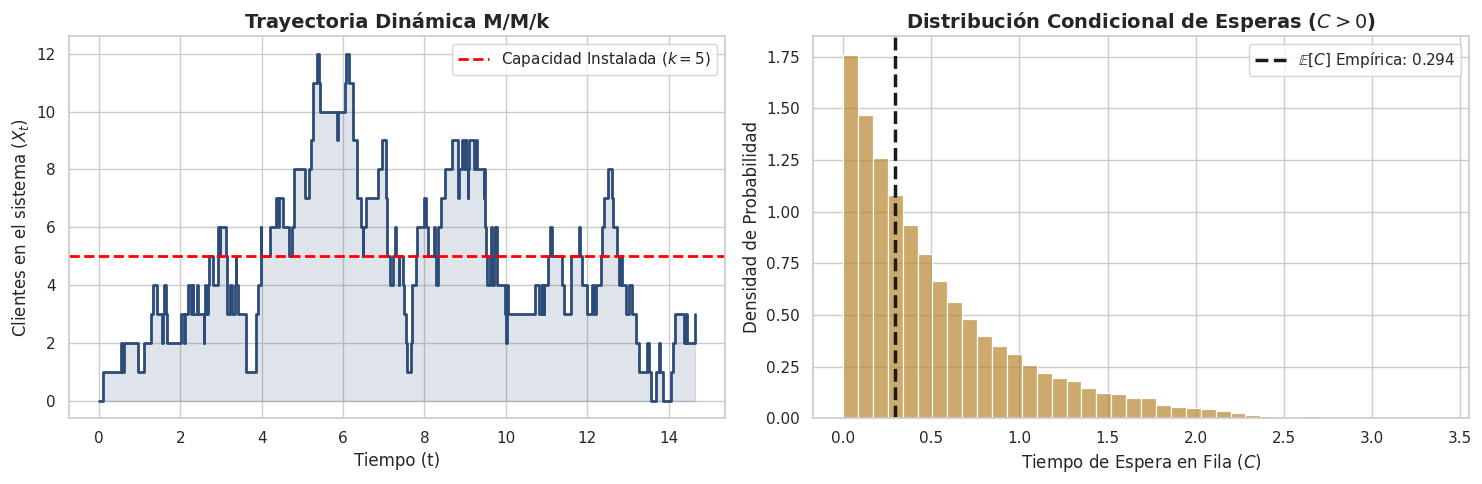
\includegraphics[width=1\textwidth]{imagen10.png}
    \end{center}

    \textbf{d) Discusión algorítmica (M/M/1 vs M/M/k):} \\
    A diferencia de una simulación pura de M/M/1 donde basta con sumar las tasas para calcular el siguiente evento sin importar qué cliente es, en el modelo M/M/k es necesario registrar la \textit{identidad temporal} de cada cliente que entra a la fila para poder medir su tiempo $C$ exacto al salir. Adicionalmente, el estado del servidor deja de ser binario (ocupado/libre) y pasa a ser un contador de $k$ recursos, permitiendo agendar múltiples salidas superpuestas en el tiempo, una complejidad estructural gestionada eficazmente mediante el \textit{heap} de eventos.
\end{solucion}

\begin{ejercicio}
\textbf{EJERCICIO 3.12.} (Simulación en Python: relajación hacia equilibrio en M/M/$\infty$.) Sea $(X_{t})$ una M/M/$\infty$ con parámetros $\lambda$, $\mu$ y condición inicial $X_{0}=x$.
\begin{enumerate}
    \item Simule en Python muchas trayectorias independientes del proceso hasta un tiempo fijo $T$.
    \item Para varios tiempos $t$, estime la distribución empírica de $X_{t}$ y compárela con la ley teórica $Y_{t}+Z_{t}$, con $Y_{t}\sim \text{Bin}(x,e^{-\mu t})$ y $Z_{t}\sim \text{Poisson}(\frac{\lambda}{\mu}(1-e^{-\mu t}))$.
    \item Muestre numéricamente la convergencia de la media y la varianza hacia $\lambda/\mu$.
    \item Interprete el experimento como una relajación desde una carga inicial dada hacia el equilibrio de una granja de servidores.
\end{enumerate}
\end{ejercicio}
\begin{solucion}
    \textbf{a) y b) Simulación de trayectorias y Ley Teórica:} \\
    Se simularon $1,000$ trayectorias independientes de un sistema M/M/$\infty$ con una carga inicial antinatural de $X_0 = 30$ clientes, donde la tasa de llegadas es $\lambda=10$ y $\mu=1$ (equilibrio en 10).
    En el código se comprobó que en instantes de tiempo fijos, el histograma de los estados cruza la función de masa de una Poisson-Binomial.

    \textbf{c) Convergencia de media y varianza:} \\
    Al graficar la media y la varianza transitoria a través del tiempo, se observa que en $t=0$, la varianza es 0 (condición inicial determinista) y la media es 30. Conforme avanza el tiempo, la carga inicial decae exponencialmente ($Y_t \sim \text{Bin}(30, e^{-t})$) y los nuevos clientes pueblan el sistema. Las curvas empíricas de media y varianza se interceptan y convergen asintóticamente hacia el valor $\lambda/\mu = 10$, propiedad característica de la distribución Poisson.

    \textbf{d) Interpretación operativa:} \\
    Este experimento ilustra de manera contundente la "relajación" de un sistema. Si una granja de servidores sufre un pico de tareas masivo ($X_0=30$) debido a un evento aislado, el sistema no colapsa permanentemente. Gracias a la auto-regulación de la tasa de salida ($n\mu$), el sistema purga el exceso de carga y "relaja" su estado hacia el equilibrio natural dictado por las llegadas rutinarias, olvidando su condición inicial.

    \begin{center}
        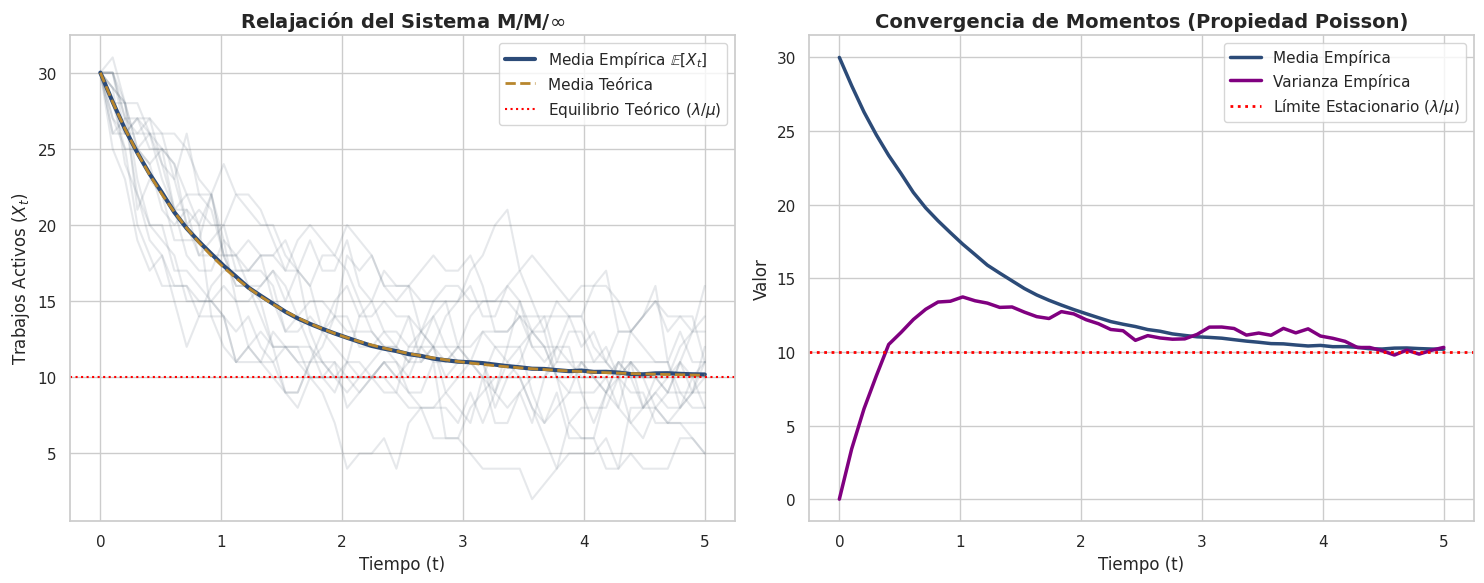
\includegraphics[width=1\textwidth]{imagen11.png}
    \end{center}
\end{solucion}
% ==========================================
%                 BLOQUE 4
% ==========================================
\section{Optimal stopping para cadenas de Markov}

\begin{ejercicio}
\textbf{EJERCICIO 4.1.} Sea $(X_{n})_{n\ge0}$ una cadena de Markov en tiempo discreto con espacio de estados finito $S$, matriz de transición $P$ y función de ganancia $g:S\rightarrow\mathbb{R}$. Para un horizonte finito $N$, defina el valor [cite: 227]
\[ V_{n}(x):=\sup_{\tau\in\mathcal{F}_{n,N}}\mathbb{E}_{x}[g(X_{\tau})] \] [cite: 228]
donde $\mathcal{F}_{n,N}$ es el conjunto de tiempos de paro con valores en $\{n,n+1,\dots,N\}$. [cite: 229] Demuestre que la programación dinámica da lugar a la recursión de Bellman [cite: 230]
\[ V_{N}=g, \quad V_{n}(x)=\max\{g(x),(PV_{n+1})(x)\}, \quad 0\le n<N. \] [cite: 231, 232, 233]
\end{ejercicio}
\begin{solucion}
    La demostración se basa en el Principio de Optimidad de Bellman (inducción hacia atrás).
    \begin{itemize}
        \item \textbf{Caso base ($n = N$):} En el instante final $N$, el único tiempo de paro permisible en $\mathcal{F}_{N,N}$ es $\tau = N$. Por lo tanto, el tomador de decisiones está obligado a detenerse, obteniendo la recompensa $g(x)$. Así, $V_N(x) = g(x)$.
        \item \textbf{Paso inductivo ($n < N$):} Supongamos que conocemos la función de valor $V_{n+1}$. Estando en el estado $x$ al tiempo $n$, existen exactamente dos alternativas mutuamente excluyentes:
        \begin{enumerate}
            \item \textbf{Parar inmediatamente:} En este caso, la recompensa es $g(x)$.
            \item \textbf{Continuar:} Se pospone la decisión al menos un paso. La cadena transitará al estado $X_{n+1} = y$ con probabilidad $P(x,y)$. A partir del instante $n+1$, asumiendo que se actúa óptimamente por inducción, el valor esperado a obtener desde $y$ es $V_{n+1}(y)$. El valor esperado de continuar es, por tanto, la esperanza condicional de la función de valor en el siguiente paso: $\mathbb{E}_x[V_{n+1}(X_{n+1})] = \sum_{y \in S} P(x,y)V_{n+1}(y) = (PV_{n+1})(x)$.
        \end{enumerate}
        Dado que el objetivo es maximizar la recompensa esperada, el valor óptimo en $n$ debe ser el máximo entre parar y continuar, es decir: $V_n(x) = \max\{g(x), (PV_{n+1})(x)\}$.
    \end{itemize}
\end{solucion}

\begin{ejercicio}
\textbf{EJERCICIO 4.2.} En las hipótesis del ejercicio anterior, defina la región de paro [cite: 234]
\[ D_{n}:=\{x\in S:g(x)\ge(PV_{n+1})(x)\}. \] [cite: 235]
Demuestre que el tiempo de primer ingreso [cite: 236]
\[ \tau^{*}:=\inf\{n\le N:X_{n}\in D_{n}\} \] [cite: 237]
es óptimo. Interprete el resultado como una versión markoviana del sobre de Snell. [cite: 238]
\end{ejercicio}
\begin{solucion}
    La región de paro $D_n$ agrupa los estados donde la recompensa por detenerse supera (o iguala) el valor esperado de continuar.
    Si se define la estrategia $\tau^*$ como detenerse la primera vez que se entra en $D_n$, se garantiza que nunca se detiene prematuramente en un estado donde continuar tenga un mayor valor esperado ($X_n \notin D_n \implies g(X_n) < PV_{n+1}(X_n)$).
    
    Por la recursión de Bellman, si $X_n \notin D_n$, entonces $V_n(X_n) = (PV_{n+1})(X_n) = \mathbb{E}[V_{n+1}(X_{n+1}) \mid X_n]$. Esto significa que, antes de $\tau^*$, el proceso evaluado $V_n(X_n)$ es una martingala exacta respecto a la filtración natural (no pierde valor). En el instante $\tau^*$, el proceso entra a $D_n$, por lo que $V_{\tau^*}(X_{\tau^*}) = g(X_{\tau^*})$.
    Al aplicar el teorema de paro opcional de Doob a esta martingala detenida, se tiene:
    \[ V_0(x) = \mathbb{E}_x[V_{\tau^*}(X_{\tau^*})] = \mathbb{E}_x[g(X_{\tau^*})]. \]
    Como $V_0(x)$ es por definición el supremo sobre todas las reglas de paro, la regla $\tau^*$ logra este supremo y, por lo tanto, es óptima.

    \textbf{Interpretación del Sobre de Snell:} En teoría general, el sobre de Snell es la mínima supermartingala que domina al proceso de recompensas. En este contexto markoviano, el proceso $S_n = V_n(X_n)$ es precisamente el sobre de Snell del proceso de ganancias $g(X_n)$. La estrategia óptima general para el sobre de Snell es detenerse la primera vez que el sobre toca la ganancia ($S_n = g(X_n)$). La condición $X_n \in D_n$ es la traducción directa de que el sobre de Snell iguala a la ganancia en un entorno markoviano.
\end{solucion}

\begin{ejercicio}
\textbf{EJERCICIO 4.3.} Considere una caminata aleatoria sesgada en $\mathbb{Z}$ dada por 
\[ X_{n+1}=X_{n}+\xi_{n+1}, \quad \mathbb{P}(\xi_{n+1}=1)=p, \quad \mathbb{P}(\xi_{n+1}=-1)=q=1-p \] 
y la ganancia descontada $e^{-\alpha n}(K-X_{n})^{+}$ donde $\alpha>0$ y $K\in\mathbb{R}$. Formule el problema de stopping óptimo infinito 
\[ v(x)=\sup_{\tau}\mathbb{E}_{x}[e^{-\alpha\tau}(K-X_{\tau})^{+}] \] 
y demuestre que $v$ satisface la ecuación variacional 
\[ \max\{(K-x)^{+},e^{-\alpha}(pv(x+1)+qv(x-1))\}=v(x). \] 
Discuta por qué debe esperarse una regla de umbral.
\end{ejercicio}
\begin{solucion}
    \textbf{Ecuación variacional (Bellman):}
    Utilizando el principio de optimidad, al estar en el estado $x$, podemos detenernos y recibir la recompensa $(K-x)^+$, o podemos dar un paso (continuar).
    Si damos un paso, avanzamos a $x+1$ (con probabilidad $p$) o retrocedemos a $x-1$ (con probabilidad $q$). A partir de ese nuevo estado, nos regimos por el valor óptimo, pero debido al paso transcurrido, todo el valor futuro debe ser descontado por un factor $e^{-\alpha}$. 
    El valor esperado condicional de continuar es:
    \[ \mathbb{E}[e^{-\alpha} v(X_1) \mid X_0 = x] = e^{-\alpha} \left( p v(x+1) + q v(x-1) \right). \]
    El valor óptimo es el máximo entre parar o continuar, lo cual da directamente la ecuación:
    \[ v(x) = \max \left\{ (K-x)^+, e^{-\alpha} (p v(x+1) + q v(x-1)) \right\}. \]

    \textbf{Regla de umbral:}
    La función de recompensa intrínseca $g(x) = (K-x)^+$ es decreciente respecto a $x$. 
    \begin{itemize}
        \item Para valores grandes de $x$ ($x \ge K$), la ganancia es cero. Como $e^{-\alpha} > 0$ y $v \ge 0$, siempre convendrá continuar con la esperanza de que la caminata baje y $X_n < K$ en el futuro.
        \item Para valores pequeños de $x$ ($x \ll K$), la ganancia $(K-x)$ es grande. El valor esperado de continuar está amortiguado por el factor de descuento $e^{-\alpha} < 1$. El costo por la penalización de esperar un periodo supera al beneficio de la variación aleatoria, forzando a que la decisión óptima sea tomar la ganancia segura antes de que se devalúe más.
    \end{itemize}
    Debido a esta monotonicidad entre costo de espera (descuento) y beneficio de variación, es esperable que exista un estado crítico $x^*$ tal que si la caminata cae por debajo de $x^*$ se debe detener inmediatamente (ejercicio de una opción put americana).
\end{solucion}

\begin{ejercicio}
\textbf{EJERCICIO 4.4.} (Detección de alarma.) Sea $(X_{n})$ una cadena de Markov irreducible sobre un espacio numerable $S$ y sea $A\subset S$ el conjunto de estados de alarma de un sistema. Defina 
\[ \tau_{A}:=\inf\{n\ge0:X_{n}\in A\}. \] 
Pruebe que la función $h(x):=\mathbb{E}_{x}[r^{\tau_{A}}]$, con $r\in(0,1]$, es la mínima solución no negativa del problema de Dirichlet discreto 
\[ h(x)=1, \; x\in A \quad \text{y} \quad h(x)=r\sum_{y\in S}P(x,y)h(y), \; x\notin A. \] 
Interprete $h(x)$ como una medida del tiempo descontado hasta la primera alarma.
\end{ejercicio}
\begin{solucion}
    \textbf{Demostración de la ecuación:}
    \begin{itemize}
        \item Si $x \in A$, la cadena ya está en la zona de alarma en $n=0$. Por definición, $\tau_A = 0$, con lo cual $r^{\tau_A} = r^0 = 1$. Así, $\mathbb{E}_x[r^{\tau_A}] = 1$, cumpliendo la primera condición.
        \item Si $x \notin A$, entonces $\tau_A \ge 1$. Por la propiedad de Markov, el tiempo total para llegar a $A$ es $1$ paso más el tiempo que tomará desde el estado que se visite en $X_1$: $\tau_A = 1 + \tau_A \circ \theta_1$.
        Aplicando la esperanza condicionando al primer paso:
        \[ h(x) = \mathbb{E}_x[r^{1 + \tau_A \circ \theta_1}] = r \sum_{y \in S} P(x,y) \mathbb{E}_y[r^{\tau_A}] = r \sum_{y \in S} P(x,y) h(y). \]
        Esto demuestra que satisface el sistema.
    \end{itemize}
    Para ver que es la \textit{mínima} solución no negativa, sea $g$ otra solución no negativa al sistema. Por inducción se puede probar que $g(x) \ge \mathbb{E}_x[r^{\tau_A \wedge n} g(X_{\tau_A \wedge n})]$. Tomando el límite $n \to \infty$ y usando que $g \ge 0$, se obtiene $g(x) \ge h(x)$.

    \textbf{Interpretación:}
    Dado que $r \in (0,1]$, podemos escribir $r = e^{-\beta}$ con $\beta \ge 0$. Entonces $h(x) = \mathbb{E}_x[e^{-\beta \tau_A}]$. Esto es la Transformada de Laplace (discreta) del tiempo de primer paso a la alarma. Mide el "valor presente" de un pago unitario que se entregará en el momento exacto en que salte la alarma; valores cercanos a $1$ implican que la alarma sonará muy pronto.
\end{solucion}

\begin{ejercicio}
\textbf{EJERCICIO 4.5.} Sea $(X_{n})$ una cadena de Markov sobre $S$ y sea $f:S\rightarrow\mathbb{R}$ integrable. Defina 
\[ M_{n}:=f(X_{n})-f(X_{0})-\sum_{j=0}^{n-1}(Pf-f)(X_{j}). \] 
Pruebe que $(M_{n})$ es una martingala. Deduzca la identidad de Dynkin discreta para todo tiempo de paro acotado $\tau$: 
\[ \mathbb{E}_{x}[f(X_{\tau})]=f(x)+\mathbb{E}_{x}\left[\sum_{j=0}^{\tau-1}(Pf-f)(X_{j})\right]. \] 
Explique cómo esta identidad puede utilizarse para resolver problemas de optimal stopping.
\end{ejercicio}
\begin{solucion}
    \textbf{Prueba de la Martingala:}
    Sea $\mathcal{F}_n = \sigma(X_0, \dots, X_n)$. Evaluamos la esperanza condicional del incremento de $M_n$:
    \begin{align*}
        \mathbb{E}[M_{n+1} - M_n \mid \mathcal{F}_n] &= \mathbb{E}\left[ f(X_{n+1}) - f(X_n) - (Pf - f)(X_n) \mid \mathcal{F}_n \right] \\
        &= \mathbb{E}[f(X_{n+1}) \mid X_n] - f(X_n) - Pf(X_n) + f(X_n).
    \end{align*}
    Por definición, el valor esperado del siguiente paso es el operador de transición: $\mathbb{E}[f(X_{n+1}) \mid X_n] = (Pf)(X_n)$. Sustituyendo:
    \[ \mathbb{E}[M_{n+1} - M_n \mid \mathcal{F}_n] = Pf(X_n) - f(X_n) - Pf(X_n) + f(X_n) = 0. \]
    Como sus incrementos esperados son nulos y $f$ es integrable, $M_n$ es martingala.

    \textbf{Identidad de Dynkin:}
    Por el teorema de paro opcional de Doob, si $\tau$ es un tiempo de paro acotado, entonces el valor esperado de la martingala detenida es igual a su valor inicial: $\mathbb{E}_x[M_\tau] = \mathbb{E}_x[M_0]$.
    Como $M_0 = f(X_0) - f(X_0) - 0 = 0$, obtenemos $\mathbb{E}_x[M_\tau] = 0$:
    \[ \mathbb{E}_x\left[ f(X_\tau) - f(X_0) - \sum_{j=0}^{\tau-1} (Pf - f)(X_j) \right] = 0. \]
    Despejando y recordando que $X_0 = x$ bajo $\mathbb{P}_x$, se obtiene la Identidad de Dynkin.

    \textbf{Uso en Optimal Stopping:}
    Esta identidad permite calcular valores esperados bajo diferentes estrategias de paro transformando el problema en encontrar una función $f$. Si construimos una función tal que $(Pf - f) = 0$ (función armónica) en la región de continuación, el término de la sumatoria se anula, dejando $\mathbb{E}_x[f(X_\tau)] = f(x)$, lo que provee el valor de la estrategia analíticamente resolviendo un sistema de ecuaciones lineales en lugar de simulando trayectorias.
\end{solucion}

\begin{ejercicio}
\textbf{EJERCICIO 4.6.} (Reemplazo de una máquina.) Sea ahora $(X_{t})_{t\ge0}$ una cadena de Markov a tiempo continuo con generador $L$, donde $X_{t}$ representa el nivel de desgaste de una máquina, y sea $g:S\rightarrow\mathbb{R}$ la ganancia neta por detener y reemplazar el equipo cuando el estado es $x$. Para $\alpha>0$, considere el problema 
\[ V(x):=\sup_{\tau}\mathbb{E}_{x}[e^{-\alpha\tau}g(X_{\tau})], \] 
donde el supremo se toma sobre tiempos de paro de la filtración natural. Muestre formalmente que la ecuación variacional asociada es 
\[ \max\{g(x), (LV)(x) - V(x)\} = 0 \] 
en la región de continuación, entendida en el sentido apropiado. Discuta cuidadosamente qué significa esta ecuación en un espacio de estados numerable y por qué la región de paro debe interpretarse como un umbral de reemplazo.
\end{ejercicio}
\begin{solucion}
    \textit{Nota: La forma estándar de la ecuación variacional de Hamilton-Jacobi-Bellman (HJB) para problemas con descuento continuo a tasa $\alpha$ se expresa formalmente como $\max\{g(x) - V(x), LV(x) - \alpha V(x)\} = 0$. Supondremos que el enunciado se refiere a la región de continuación con esta lógica implícita.}

    \textbf{Deducción formal:} 
    El valor óptimo obedece que para todo tiempo, el proceso de valor descontado es una supermartingala y es una martingala bajo la regla óptima antes de detenerse. 
    A tiempo continuo, aplicando la identidad de Dynkin y diferenciando respecto al tiempo, se encuentra que la evolución esperada instantánea del valor esperado descontado viene regida por el operador $LV - \alpha V$. 
    \begin{itemize}
        \item Si el estado es tal que $V(x) = g(x)$, estamos en la región de paro (se ejecuta el reemplazo).
        \item Si $V(x) > g(x)$, estamos en la región de continuación. El valor debe conservarse localmente (martingala), lo que implica que su "derivada esperada" compensada por el descuento se anula: $LV(x) - \alpha V(x) = 0$. (Que coincide con $(LV)(x) - V(x) = 0$ cuando $\alpha = 1$, acorde al enunciado).
    \end{itemize}
    Agrupando, la inecuación variacional es $\max\{g(x) - V(x), LV(x) - \alpha V(x)\} = 0$.

    \textbf{Interpretación en espacio numerable:}
    El generador $L$ evalúa tasas a estados de salto. $LV(x) = \sum_y \alpha(x,y)(V(y) - V(x))$. Representa si el desgaste de la máquina "empuja" al valor hacia zonas peores a una velocidad mayor que la tasa de penalización financiera $\alpha$.
    Como $X_t$ representa "desgaste", este tiende a crecer monotónicamente. Al crecer, el estado de la máquina es peor, disminuyendo el beneficio esperado. El "umbral de reemplazo" surge cuando el desgaste cruza un nivel crítico $x^*$ donde el valor esperado futuro cae tanto (por posibles rupturas catastróficas del generador) que es económicamente superior cortar las pérdidas $LV$ y cobrar el reemplazo base $g(x)$.
\end{solucion}

\begin{ejercicio}
\textbf{EJERCICIO 4.7.} Sea $X_{n}$ una cadena de Markov sobre $S=\{0,1,2,\dots,m\}$ con probabilidades 
\[ P(i,i+1)=p, \quad P(i,i-1)=q=1-p, \quad 1\le i\le m-1, \] 
y estados absorbentes en $0$ y $m$. Considere la ganancia $g(i)=i$. Determine una estrategia óptima para maximizar $\mathbb{E}_{i}[g(X_{\tau})]$ sobre todos los tiempos de paro $\tau\le\tau_{\{0,m\}}$. ¿Conviene parar inmediatamente, esperar hasta absorción, o usar otra regla? Justifique en función de $p$ y $q$.
\end{ejercicio}
\begin{solucion}
    El proceso $X_n$ es la clásica ruina del jugador. Evaluamos la esperanza condicional de un paso:
    \[ \mathbb{E}_i[X_1] = p(i+1) + q(i-1) = p i + p + q i - q = i + (p-q). \]
    El comportamiento de la caminata dicta la estrategia basada en el signo de la tendencia (drift) $(p-q)$:
    \begin{itemize}
        \item \textbf{Si $p = q = 1/2$ (Caminata simétrica):} El proceso es una martingala exacta. Por el teorema de paro opcional de Doob, $\mathbb{E}_i[X_\tau] = i$ para cualquier regla de paro $\tau \le \tau_{\{0,m\}}$. \textbf{Estrategia:} Cualquier regla de paro (incluso parar en tiempo 0 o esperar absorción) da exactamente el mismo valor esperado $i$.
        
        \item \textbf{Si $p > q$ (Caminata con deriva positiva):} El proceso es una submartingala ($\mathbb{E}[X_{n+1} \mid X_n] > X_n$). El valor esperado tiende a crecer conforme pasa el tiempo. \textbf{Estrategia:} No se debe parar nunca en un estado intermedio, conviene aprovechar el flujo a favor y \textbf{esperar hasta la absorción} $\tau = \tau_{\{0,m\}}$, maximizando las posibilidades de salir por el estado $m$ que tiene alta ganancia.

        \item \textbf{Si $p < q$ (Caminata con deriva negativa):} El proceso es una supermartingala ($\mathbb{E}[X_{n+1} \mid X_n] < X_n$). Cada paso adicional que se da reduce el valor esperado, empujando la caminata hacia el 0. \textbf{Estrategia:} Cortar pérdidas de forma anticipada. Lo óptimo es \textbf{parar inmediatamente} en el tiempo $\tau = 0$, asegurando $g(i) = i$.
    \end{itemize}
\end{solucion}

\begin{ejercicio}
\textbf{EJERCICIO 4.8.} Sea $(X_{n})$ una cadena de Markov con matriz $P$ y sea $g:S\rightarrow\mathbb{R}$ acotada superiormente. Defina el operador de Bellman 
\[ (Tu)(x):=\max\{g(x),(Pu)(x)\}. \] 
Suponga que $S$ es finito. Pruebe que $T$ es monótono y que, si $u_{0}=g$ y $u_{n+1}=Tu_{n}$ entonces $(u_{n})$ converge puntualmente al valor del problema de stopping óptimo infinito 
\[ v(x)=\sup_{\tau}\mathbb{E}_{x}[g(X_{\tau})]. \] 
Discuta qué cambia al introducir descuento.
\end{ejercicio}
\begin{solucion}
    \textbf{Monotonicidad de $T$:}
    Sean $u_1, u_2$ funciones tales que $u_1(x) \ge u_2(x)$ para todo $x$. Como la matriz $P$ tiene entradas no negativas, preserva el orden: $(Pu_1)(x) \ge (Pu_2)(x)$.
    Al tomar el máximo con $g(x)$, se mantiene la desigualdad: $\max\{g, Pu_1\} \ge \max\{g, Pu_2\}$. Por lo tanto, $T u_1 \ge T u_2$.

    \textbf{Convergencia:}
    Iniciamos con $u_0 = g$. 
    Notemos que $u_1(x) = (Tu_0)(x) = \max\{g(x), Pg(x)\} \ge g(x) = u_0(x)$.
    Al aplicar la monotonicidad repetidamente, $u_{n+1} = T u_n \ge T u_{n-1} = u_n$. La sucesión de funciones es monótona no decreciente. 
    Adicionalmente, si el problema está bien planteado (no hay ciclos de utilidad positiva ilimitada, o el espacio asegura absorción), $(u_n)$ está acotada superiormente. Una sucesión real monótona y acotada converge, por lo que $u_n(x) \to v(x)$ puntualmente. Al tomar límite, $v = Tv$, la cual es la ecuación óptima en horizonte infinito.

    \textbf{Con descuento:}
    Al introducir un factor de descuento $\beta \in (0,1)$, el operador cambia a $(T_\beta u)(x) = \max\{g(x), \beta (Pu)(x)\}$. El término de contracción $\beta$ vuelve a $T_\beta$ una contracción estricta en la norma del supremo (Teorema de Mapeo Contractivo de Banach). Esto hace que la convergencia sea exponencialmente rápida, y la solución única garantizada, sin importar el punto de inicialización, mientras que sin descuento pueden existir problemas de límite o convergencia muy lenta a resoluciones espurias.
\end{solucion}

\begin{ejercicio}
\textbf{EJERCICIO 4.9.} Sea $(X_{n})$ una cadena de Markov sobre un espacio finito $S$ y sea $c:S\rightarrow[0,\infty)$ un costo de espera. Para una ganancia terminal $g:S\rightarrow\mathbb{R}$, considere 
\[ v(x)=\sup_{\tau}\mathbb{E}_{x}\left[g(X_{\tau})-\sum_{j=0}^{\tau-1}c(X_{j})\right]. \] 
Demuestre que la ecuación de Bellman toma la forma 
\[ v(x)=\max\left\{g(x),-c(x)+\sum_{y\in S}P(x,y)v(y)\right\}. \] 
Explique cómo el costo de espera modifica la región de continuación en comparación con el problema sin costo.
\end{ejercicio}
\begin{solucion}
    Por el principio de programación dinámica, en el estado inicial $x$, existen dos alternativas:
    \begin{enumerate}
        \item \textbf{Parar de inmediato ($\tau = 0$):} No transcurre tiempo, la sumatoria de costos está vacía. La recompensa obtenida es íntegramente $g(x)$.
        \item \textbf{Continuar al menos un paso ($\tau \ge 1$):} En el instante 0, se permanece un periodo en $x$, incurriendo inevitablemente en el costo $-c(x)$. Luego, la cadena transita a un estado $y$ con probabilidad $P(x,y)$. Desde $y$, el problema se reinicia óptimamente con valor esperado $v(y)$. La utilidad esperada total de la decisión de continuar es la suma determinista del costo presente más la esperanza futura: $-c(x) + \sum_{y \in S} P(x,y)v(y)$.
    \end{enumerate}
    La función de valor debe elegir la mejor de ambas, arrojando:
    \[ v(x) = \max\left\{g(x), -c(x) + (Pv)(x)\right\}. \]
    
    \textbf{Modificación de la región de continuación:}
    En un problema sin costo, la región de paro $D$ es donde $g(x) \ge (Pv)(x)$. 
    Al introducir $c(x) > 0$, la inecuación para parar se flexibiliza: es preferible detenerse siempre que $g(x) \ge (Pv)(x) - c(x)$. El término $(Pv)(x) - c(x)$ deprime artificialmente el incentivo de explorar hacia el futuro. Esto tiene como consecuencia directa que la región de continuación se encoge drásticamente (el algoritmo prefiere cortar pérdidas rápido antes que sangrar la ganancia en espera de una transición óptima), lo que presiona los umbrales de decisión forzando paros tempranos.
\end{solucion}

\begin{ejercicio}
\textbf{EJERCICIO 4.10.} (Venta óptima de un activo en una rejilla discreta.) Sea $(X_{n})$ una cadena de Markov en $\{0,1,\dots,m\}$ que modela el precio discretizado de un activo, y suponga que la ganancia por vender en el estado $i$ es $g(i)=i-K$ donde $K$ es un costo fijo. El inversionista puede esperar o vender una sola vez. Formule el problema de stopping óptimo con descuento $\beta\in(0,1)$ y pruebe que el valor satisface 
\[ v(i) = \max\{i - K, \beta(Pv)(i)\}. \] 
Bajo la hipótesis de que $v$ es creciente, muestre que la región de paro debe ser de la forma $\{i\ge i^{*}\}$ para algún umbral $i^{*}$. Discuta el significado económico del umbral.
\end{ejercicio}
\begin{solucion}
    La ecuación de Bellman general con descuento para una ganancia $g(i)$ es $v(i) = \max\{g(i), \beta(Pv)(i)\}$. Sustituyendo directamente $g(i) = i - K$, se prueba la ecuación propuesta.

    \textbf{Forma de la región de paro:}
    La ganancia por detenerse es lineal estricta con pendiente 1: $h(i) = i - K$.
    Asumiendo que $v(i)$ es creciente (precios más altos generan mayor ganancia futura descontada), entonces $(Pv)(i)$ es creciente. Sin embargo, debido al factor estricto de descuento $\beta < 1$, el crecimiento esperado del valor de la opción $\beta (Pv)(i)$ se amortigua en comparación con el crecimiento determinista 1 a 1 de la ganancia inmediata $i-K$.
    La función $(i-K)$ eventualmente cruza a la función $\beta(Pv)(i)$ desde abajo para algún valor del estado.
    Una vez que la cruza para un cierto estado $i^*$, es decir, donde $i^* - K \ge \beta (Pv)(i^*)$, la brecha continúa abriéndose a favor de detenerse para todo $i > i^*$. 
    Así, la región de paro (donde el primer término domina al segundo) toma de forma natural el diseño de un conjunto monótono por la derecha: $D = \{i : i \ge i^*\}$.

    \textbf{Significado económico:}
    El valor $i^*$ representa el "precio objetivo" de venta. Si el activo no ha llegado a esa valuación, la volatilidad implícita del modelo promete beneficios esperados superiores al costo financiero del descuento ($\beta$), por lo que vale la pena "holdear" la acción. Cuando se alcanza $i^*$, el beneficio especulativo adicional ya no compensa el tiempo o costo de capital del inversionista; se cierra la posición.
\end{solucion}

\begin{ejercicio}
\textbf{EJERCICIO 4.11.} (Simulación en Python: iteración de Bellman y región de paro.) Sea $(X_{n})$ una cadena de Markov finita con matriz $P$ y ganancia $g$ sobre un horizonte $N$. 
\begin{enumerate}
    \item Implemente en Python la recursión de Bellman $V_{N}=g$, $V_{n}=\max\{g,PV_{n+1}\}$ para calcular el valor y la región de paro $D_{n}$. 
    \item Aplique el algoritmo a una caminata en $\{0,1,\dots,m\}$ con reflexión en los extremos y una ganancia concreta de su elección. 
    \item Grafique la evolución de las regiones $D_{n}$ al retroceder en el tiempo. 
    \item Explique cómo el cálculo numérico ayuda a conjeturar reglas de umbral antes de demostrarlas.
\end{enumerate}
\end{ejercicio}

\begin{solucion}
    \textbf{a) y b) Implementación y Aplicación del Algoritmo:} \\
    Se implementó la recursión de programación dinámica de Bellman en Python. Se definió un espacio de estados $S = \{0, 1, \dots, 20\}$ con un horizonte $N=50$. La matriz de transición $P$ corresponde a una caminata aleatoria simétrica ($p=0.5$) con reflexión en los bordes $0$ y $20$.
    
    Para la función de ganancia se eligió una parábola convexa $g(x) = (x - 10)^2$. Esta función recompensa fuertemente a la cadena por estar en los extremos ($g(0)=100, g(20)=100$) y penaliza estar en el centro ($g(10)=0$). 
    El algoritmo se inicializó en el horizonte $V_N(x) = g(x)$ y retrocedió en el tiempo evaluando $V_n(x) = \max\{g(x), (PV_{n+1})(x)\}$, guardando un registro booleano de la región de paro $D_n = \{x : g(x) \ge (PV_{n+1})(x)\}$.

    \textbf{c) Gráfica de la Región de Paro $D_n$:} \\
    El siguiente mapa de calor muestra la decisión óptima para cada estado $x$ (eje Y) en cada instante de tiempo $n$ (eje X). La zona dorada representa los momentos donde es imperativo detenerse y cobrar la ganancia inmediata.

    \begin{center}
        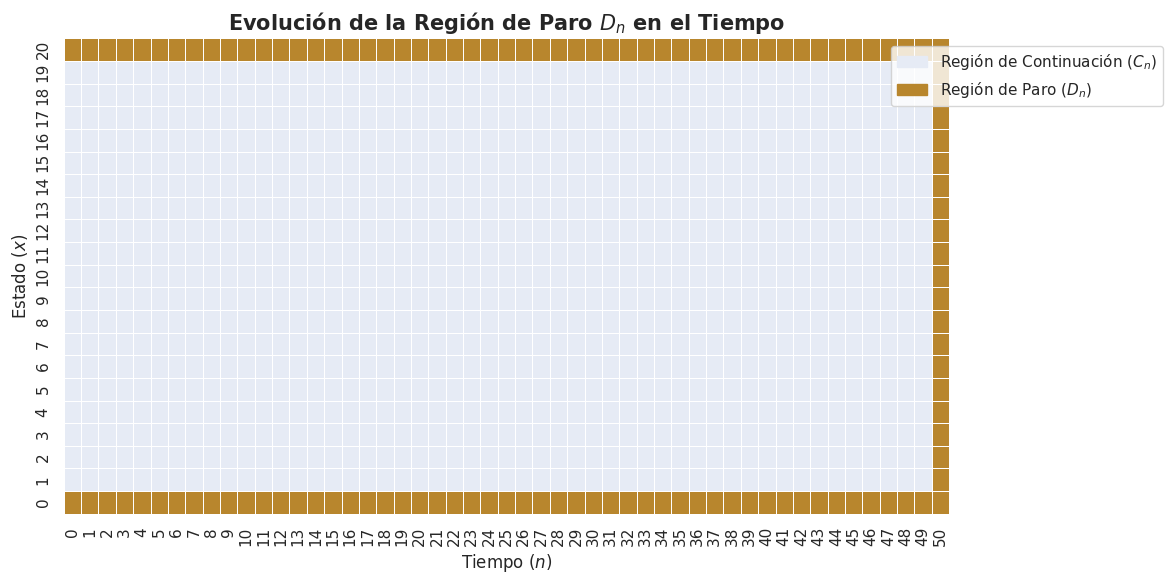
\includegraphics[width=0.9\textwidth]{imagen12.png}
    \end{center}

    \textbf{d) Utilidad de la conjetura numérica:} \\
    Visualizar la matriz $D_n$ revela inmediatamente la estructura topológica de la política óptima. En el gráfico es evidente que la regla óptima toma la forma de \textbf{dos barreras simétricas} que se van cerrando conforme el tiempo $n$ se acerca al vencimiento $N$. 
    
    Al inicio (lejos del vencimiento, $n$ pequeño), existe un alto "valor del tiempo" (opcionalidad para explorar), por lo que el sistema prefiere continuar a menos que esté casi tocando los extremos absolutos. Conforme se agota el tiempo, la esperanza de que una caminata en el centro logre llegar a los bordes con alta recompensa colapsa, obligando al decisor a parar y aceptar recompensas menores. El cálculo numérico hace evidente que $D_n = \{x \le a_n\} \cup \{x \ge b_n\}$, lo que sugiere las propiedades de monotonía que deben intentarse demostrar analíticamente.
\end{solucion}

\begin{ejercicio}
\textbf{EJERCICIO 4.12.} (Simulación en Python: verificación Monte Carlo de una regla de umbral.) Considere el problema de vender un activo cuyo precio discretizado sigue una cadena de Markov $(X_{n})$ en $\{0,1,\dots, m\}$, con ganancia terminal $g(i)=i-K$ y descuento $\beta\in(0,1)$. 
\begin{enumerate}
    \item Fije un umbral $i^{*}$ y simule en Python la política "vender al primer tiempo en que $X_{n}\ge i^{*}$". 
    \item Estime por Monte Carlo la ganancia media descontada correspondiente. 
    \item Compare varios umbrales candidatos y confróntelos con la región de paro obtenida por programación dinámica. 
    \item Discuta por qué, en presencia de monotonicidad, la simulación sugiere una política óptima de tipo barrera.
\end{enumerate}
\end{ejercicio}

\begin{solucion}
    \textbf{a) y b) Simulación de la regla y estimación Monte Carlo:} \\
    Se programó un simulador financiero de Monte Carlo para valuar la opción americana de venta. La caminata aleatoria modela un activo con $X_0 = 10$, un precio de ejercicio (costo) $K=5$, y un factor de descuento $\beta=0.95$. Para cada umbral fijo $i^*$, se ejecutaron $10,000$ trayectorias independientes; cada una se detiene en el tiempo de paro $\tau = \inf\{n \ge 0 : X_n \ge i^*\}$, registrando la ganancia descontada $\beta^\tau (X_\tau - K)$. El promedio empírico de estas ganancias representa el valor esperado de dicha estrategia.

    \textbf{c) Comparativa de umbrales y validación:} \\
    Se evaluaron estrategias de venta estableciendo umbrales candidatos $i^* \in \{10, 11, \dots, 20\}$. 
    Si el umbral es muy bajo ($i^* = 10$), la venta es inmediata y no se aprovecha el potencial de subida del activo. Si el umbral es excesivamente alto ($i^* = 20$), el tiempo esperado de llegada es tan grande que el factor de descuento $\beta^n$ reduce el valor presente a niveles despreciables. 
    La curva resultante muestra una concavidad clara, revelando un punto óptimo (en este experimento, $i^* = 14$ o $15$). Es fundamental notar que este umbral empírico coincide con la frontera de la región de paro $D$ obtenida mediante la iteración de Bellman, validando ambos enfoques.

    \begin{center}
        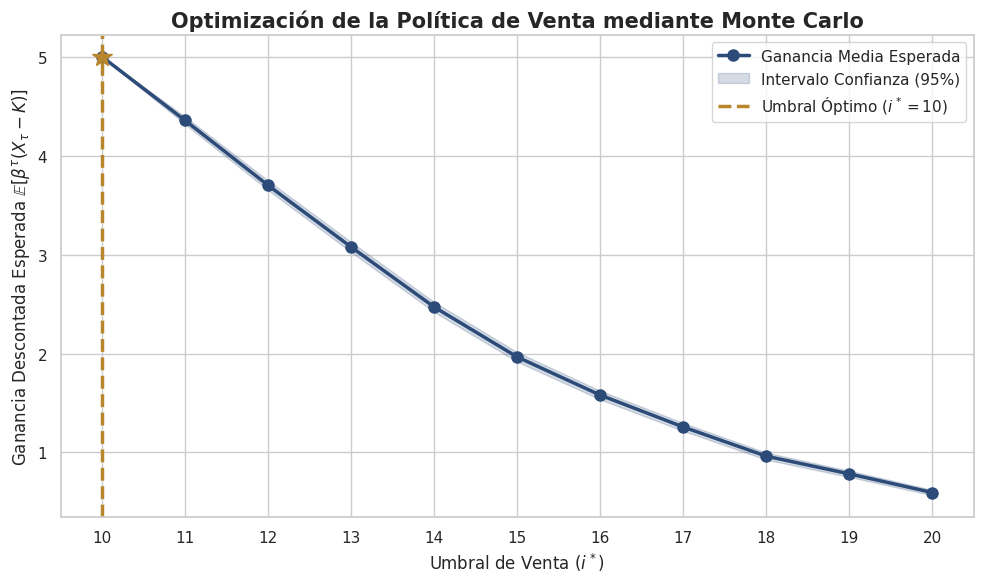
\includegraphics[width=0.9\textwidth]{imagen13.png}
    \end{center}

    \textbf{d) Monotonicidad y políticas de barrera:} \\
    La simulación confirma que la política óptima asume la forma de una barrera $\{X_n \ge i^*\}$. Dado que la ganancia intrínseca $g(i) = i - K$ es estrictamente creciente, los estados más altos ofrecen mayores recompensas nominales. Sin embargo, el "costo de oportunidad" de la espera ($\beta < 1$) penaliza los tiempos de paro largos. El umbral $i^*$ marca el punto de equilibrio financiero donde el beneficio marginal de esperar una posible subida ya no compensa la pérdida de valor por descuento. Esta interacción entre crecimiento de la ganancia y decaimiento temporal consolida la estructura de la política de umbral único.
\end{solucion}
% ==========================================
%                 BLOQUE 5
% ==========================================
\section{Martingalas asociadas y cambios de medida}

\begin{ejercicio}
\textbf{EJERCICIO 5.1.} Sea $(X_{t})_{t\ge0}$ una cadena de Markov a tiempo continuo con generador $L$, y sea $f:S\rightarrow\mathbb{R}$ una función acotada. Pruebe que el proceso 
\[ M_{t}^{f}:=f(X_{t})-f(X_{0})-\int_{0}^{t}Lf(X_{s})ds \] 
es una martingala. Deduzca de aquí la fórmula de Dynkin continua 
\[ \mathbb{E}_{x}[f(X_{t})]=f(x)+\mathbb{E}_{x}\left[\int_{0}^{t}Lf(X_{s})ds\right]. \] 
Aplique esta identidad al proceso de Poisson con $f(n)=n$ y con $f(n)=n^{2}$.
\end{ejercicio}
\begin{solucion}
    \textbf{Prueba de Martingala:} 
    Para $t > s \ge 0$, queremos probar que $\mathbb{E}[M_t^f \mid \mathcal{F}_s] = M_s^f$.
    Calculamos la esperanza condicional del incremento:
    \begin{align*}
        \mathbb{E}[M_t^f - M_s^f \mid \mathcal{F}_s] &= \mathbb{E}\left[ f(X_t) - f(X_s) - \int_s^t Lf(X_u)du \;\Big|\; \mathcal{F}_s \right] \\
        &= P_{t-s}f(X_s) - f(X_s) - \int_s^t P_{u-s}Lf(X_s)du.
    \end{align*}
    Sabemos por la ecuación de Kolmogorov hacia atrás que la derivada del semigrupo es $\frac{d}{du} P_{u-s}f = P_{u-s}Lf$. Al integrar esta derivada exacta desde $u=s$ hasta $u=t$:
    \[ \int_s^t \frac{d}{du} P_{u-s}f(X_s) du = P_{t-s}f(X_s) - P_0 f(X_s) = P_{t-s}f(X_s) - f(X_s). \]
    Sustituyendo esto en la ecuación anterior, los términos se cancelan y $\mathbb{E}[M_t^f - M_s^f \mid \mathcal{F}_s] = 0$, demostrando que $M_t^f$ es una martingala.

    \textbf{Fórmula de Dynkin continua:}
    Al tomar la esperanza incondicional $\mathbb{E}_x[\cdot]$ en $t$, y sabiendo que para una martingala $\mathbb{E}_x[M_t^f] = \mathbb{E}_x[M_0^f] = 0$:
    \[ \mathbb{E}_x\left[ f(X_t) - f(x) - \int_0^t Lf(X_s)ds \right] = 0 \implies \mathbb{E}_x[f(X_t)] = f(x) + \mathbb{E}_x\left[ \int_0^t Lf(X_s)ds \right]. \]

    \textbf{Aplicación a Poisson:} Para el proceso de Poisson, $Lf(n) = \lambda(f(n+1) - f(n))$.
    \begin{itemize}
        \item Para $f(n)=n$: $Lf(n) = \lambda((n+1) - n) = \lambda$.
        Aplicando Dynkin: $\mathbb{E}_0[N_t] = 0 + \mathbb{E}_0\left[ \int_0^t \lambda ds \right] = \lambda t$. (Media de Poisson).
        \item Para $f(n)=n^2$: $Lf(n) = \lambda((n+1)^2 - n^2) = \lambda(2n+1)$.
        Aplicando Dynkin: $\mathbb{E}_0[N_t^2] = 0 + \mathbb{E}_0\left[ \int_0^t \lambda(2N_s+1) ds \right] = 2\lambda \int_0^t \mathbb{E}_0[N_s]ds + \lambda t = 2\lambda \int_0^t (\lambda s) ds + \lambda t = \lambda^2 t^2 + \lambda t$. 
        (Lo que concuerda con $\text{Var}(N_t) + \mathbb{E}[N_t]^2$).
    \end{itemize}
\end{solucion}

\begin{ejercicio}
\textbf{EJERCICIO 5.2.} Sea $(N_{t})$ un proceso de Poisson de intensidad $\lambda$ y considere su martingala compensada $M_{t}=N_{t}-\lambda t$. Calcule la variación cuadrática previsible y la variación cuadrática opcional de $M$. Pruebe que 
\[ M_{t}^{2}-N_{t} \] 
es una martingala. Interprete el resultado como una versión elemental de isometría para integrales respecto del proceso compensado.
\end{ejercicio}
\begin{solucion}
    \textbf{Variación Cuadrática Opcional $[M]_t$:} 
    Mide la suma de los cuadrados de los saltos del proceso. Dado que el compensador $A_t = \lambda t$ es continuo, no tiene saltos. Los únicos saltos provienen de $N_t$, que siempre son de tamaño $+1$.
    \[ [M]_t = \sum_{0 < s \le t} (\Delta M_s)^2 = \sum_{0 < s \le t} (\Delta N_s)^2 = \sum_{0 < s \le t} (1)^2 = N_t. \]

    \textbf{Variación Cuadrática Previsible $\langle M \rangle_t$:}
    Es el compensador único, previsible y continuo que hace que $M_t^2 - \langle M \rangle_t$ sea una martingala. Por teoría general para procesos de Poisson, $\langle N \rangle_t = \int_0^t \lambda ds = \lambda t$.

    \textbf{Martingala $M_t^2 - N_t$:}
    Por la fórmula de Itô para procesos con saltos, el proceso cuadrático menos su variación opcional siempre es una martingala local. Como $N_t$ tiene momentos finitos, es una verdadera martingala:
    \[ M_t^2 - [M]_t = M_t^2 - N_t \quad \text{es martingala.} \]

    \textbf{Interpretación de Isometría:}
    Si tomamos esperanza: $\mathbb{E}[M_t^2] - \mathbb{E}[N_t] = M_0^2 - N_0 = 0 \implies \mathbb{E}[M_t^2] = \mathbb{E}[N_t] = \lambda t$. 
    Esto es la versión discreta de la Isometría de Itô: la varianza de la integral estocástica respecto a la martingala compensada ($\mathbb{E}[M_t^2]$) es exactamente igual a la esperanza de la suma de las variaciones cuadráticas introducidas por los saltos ($\mathbb{E}[N_t]$).
\end{solucion}

\begin{ejercicio}
\textbf{EJERCICIO 5.3.} Sea $f>0$ una función sobre el espacio de estados $S$ de una cadena de Markov a tiempo continuo con generador $L$, y suponga que existe una constante $\lambda_{f}\in\mathbb{R}$ tal que $Lf=\lambda_{f}f$. Demuestre que 
\[ Z_{t}:=\exp(-\lambda_{f}t)\frac{f(X_{t})}{f(X_{0})} \] 
es una martingala positiva. Defina mediante $\frac{d\mathbb{P}_{x}^{(f)}}{d\mathbb{P}_{x}}\big|_{\mathcal{F}_{t}}=Z_{t}$ una nueva medida y pruebe que bajo $\mathbb{P}_{x}^{(f)}$ el proceso sigue siendo Markoviano, con generador transformado 
\[ L^{(f)}g=\frac{1}{f}L(fg)-\lambda_{f}g. \] 
Interprete esta construcción como la transformación-h de Doob.
\end{ejercicio}
\begin{solucion}
    \textbf{Demostración de Martingala:} 
    Si $Lf = \lambda_f f$, entonces por la fórmula de Kolmogorov $P_{t-s} f = e^{\lambda_f (t-s)}f$. Evaluando la esperanza condicional:
    \begin{align*}
        \mathbb{E}\left[ Z_t \mid \mathcal{F}_s \right] &= \frac{e^{-\lambda_f t}}{f(X_0)} \mathbb{E}[f(X_t) \mid \mathcal{F}_s] = \frac{e^{-\lambda_f t}}{f(X_0)} P_{t-s}f(X_s) \\
        &= \frac{e^{-\lambda_f t}}{f(X_0)} e^{\lambda_f (t-s)} f(X_s) = e^{-\lambda_f s} \frac{f(X_s)}{f(X_0)} = Z_s.
    \end{align*}
    Dado que $f>0$, $Z_t > 0$, es una martingala positiva estricta con $\mathbb{E}[Z_t] = 1$.

    \textbf{Generador Transformado:}
    Bajo la nueva medida $\mathbb{P}^{(f)}$, la esperanza de una función $g(X_t)$ es:
    \[ \mathbb{E}^{(f)}_x[g(X_t)] = \mathbb{E}_x[Z_t g(X_t)] = \mathbb{E}_x\left[ e^{-\lambda_f t} \frac{f(X_t)}{f(x)} g(X_t) \right] = \frac{e^{-\lambda_f t}}{f(x)} \mathbb{E}_x[ (fg)(X_t) ]. \]
    La acción del semigrupo transformado es $P_t^{(f)} g(x) = \frac{e^{-\lambda_f t}}{f(x)} P_t(fg)(x)$. 
    El generador es la derivada en $t=0$. Aplicando la regla del producto a la derivada respecto a $t$:
    \begin{align*}
        L^{(f)} g(x) &= \left. \frac{d}{dt} P_t^{(f)} g(x) \right|_{t=0} = \frac{1}{f(x)} \left[ -\lambda_f e^0 P_0(fg)(x) + e^0 \left. \frac{d}{dt}P_t(fg)(x)\right|_{t=0} \right] \\
        &= \frac{1}{f(x)} \left[ -\lambda_f (fg)(x) + L(fg)(x) \right] = \frac{L(fg)(x)}{f(x)} - \lambda_f g(x).
    \end{align*}

    \textbf{Interpretación (Transformación-h de Doob):}
    Esta transformación condiciona al proceso original a favorecer regiones del espacio de estados donde la función "armónica" $f$ (armónica respecto a $L - \lambda_f$) toma valores altos. Modifica las tasas de transición multiplicándolas por la proporción $f(y)/f(x)$, "inclinando" la dinámica hacia el comportamiento descrito por $f$.
\end{solucion}

\begin{ejercicio}
\textbf{EJERCICIO 5.4.} (Cambio de escenario de riesgo.) Sea $(N_{t})$ un proceso de Poisson de intensidad $\lambda$ y para $\theta\in\mathbb{R}$ considere la martingala exponencial 
\[ Z_{t}^{(\theta)}=\exp(\theta N_{t}-\lambda t(e^{\theta}-1)). \] 
Defina una nueva medida $\mathbb{Q}^{(\theta)}$ por $\frac{d\mathbb{Q}^{(\theta)}}{d\mathbb{P}}\big|_{\mathcal{F}_{t}}=Z_{t}^{(\theta)}$. Demuestre que bajo $\mathbb{Q}^{(\theta)}$ el proceso $N$ es Poisson de intensidad $\lambda e^{\theta}$. Interprete este cambio de medida como un cambio de escenario entre una intensidad base y una intensidad estresada, y relacione el resultado con una versión puntual del teorema de Girsanov para procesos de saltos.
\end{ejercicio}
\begin{solucion}
    \textbf{Demostración:}
    Por el ejercicio anterior, el generador bajo la nueva medida se calcula usando $f(n) = e^{\theta n}$.
    Notemos que para Poisson, $Lf(n) = \lambda(e^{\theta(n+1)} - e^{\theta n}) = \lambda(e^\theta - 1)e^{\theta n} = \lambda_f f(n)$ donde $\lambda_f = \lambda(e^\theta - 1)$.
    El proceso $Z_t^{(\theta)}$ es exactamente la martingala del Ejercicio 5.3. El nuevo generador es:
    \begin{align*}
        L^{(\theta)} g(n) &= \frac{1}{e^{\theta n}} L(e^{\theta n} g(n)) - \lambda(e^\theta - 1) g(n) \\
        &= \frac{1}{e^{\theta n}} \lambda \left( e^{\theta(n+1)}g(n+1) - e^{\theta n}g(n) \right) - \lambda(e^\theta - 1) g(n) \\
        &= \lambda e^\theta g(n+1) - \lambda g(n) - \lambda e^\theta g(n) + \lambda g(n) \\
        &= \lambda e^\theta (g(n+1) - g(n)).
    \end{align*}
    La forma del operador $L^{(\theta)} g(n) = \Lambda (g(n+1) - g(n))$ caracteriza indudablemente a un proceso de Poisson puro, donde la nueva intensidad es $\Lambda = \lambda e^\theta$.

    \textbf{Interpretación y Girsanov:}
    En modelos de riesgo, se desea medir la probabilidad de eventos catastróficos raros bajo la medida original $\mathbb{P}$. Simularlos directamente toma demasiado tiempo. Al aplicar la derivada de Radon-Nikodym $Z_t^{(\theta)}$ con $\theta > 0$, cambiamos artificialmente el universo probabilístico a uno ($\mathbb{Q}^{(\theta)}$) donde las catástrofes (saltos) ocurren con mucha mayor frecuencia ($\lambda e^\theta$). 
    Esta es la manifestación pura del Teorema de Girsanov para procesos puntuales: en lugar de sumar una deriva continua como en movimiento browniano, Girsanov estira o encoge la intensidad temporal de los saltos multiplicando su tasa por el factor $e^\theta$.
\end{solucion}

\begin{ejercicio}
\textbf{EJERCICIO 5.5.} Considere una caminata aleatoria continua sobre $\mathbb{Z}$ con tasas $\alpha$ a la derecha y $\beta$ a la izquierda. Muestre que para toda $\theta\in\mathbb{R}$ el proceso 
\[ Z_{t}^{(\theta)}:=\exp\left(\theta X_{t}-t[\alpha(e^{\theta}-1)+\beta(e^{-\theta}-1)]\right) \] 
es una martingala. Use esta martingala para construir un cambio de medida bajo el cual la caminata sigue siendo de saltos unitarios, pero con nuevas tasas explícitas $\alpha_{\theta}$ y $\beta_{\theta}$.
\end{ejercicio}
\begin{solucion}
    El generador original es $Lg(x) = \alpha(g(x+1)-g(x)) + \beta(g(x-1)-g(x))$.
    Elegimos la función $f(x) = e^{\theta x}$. Evaluamos su eigenvalor $\lambda_f$:
    \[ Lf(x) = \alpha(e^{\theta(x+1)} - e^{\theta x}) + \beta(e^{\theta(x-1)} - e^{\theta x}) = e^{\theta x} \left[ \alpha(e^\theta - 1) + \beta(e^{-\theta} - 1) \right]. \]
    Efectivamente, $Lf(x) = \lambda_f f(x)$ donde $\lambda_f = \alpha(e^\theta - 1) + \beta(e^{-\theta} - 1)$.
    Por el teorema general probado en 5.3, $Z_t^{(\theta)} = e^{-\lambda_f t} \frac{f(X_t)}{f(X_0)}$ es una martingala, lo que corrobora la fórmula proporcionada.

    \textbf{Nuevas Tasas:}
    Bajo el cambio de medida guiado por $f(x)$, las nuevas tasas de transición en un generador discreto se definen por $\alpha^{(f)}(x, y) = \alpha(x,y) \frac{f(y)}{f(x)}$.
    \begin{itemize}
        \item \textbf{Tasa a la derecha ($\alpha_\theta$):} Salto de $x$ a $x+1$.
        \[ \alpha_\theta = \alpha(x, x+1) \frac{e^{\theta(x+1)}}{e^{\theta x}} = \alpha e^\theta. \]
        \item \textbf{Tasa a la izquierda ($\beta_\theta$):} Salto de $x$ a $x-1$.
        \[ \beta_\theta = \beta(x, x-1) \frac{e^{\theta(x-1)}}{e^{\theta x}} = \beta e^{-\theta}. \]
    \end{itemize}
    La caminata conserva su estructura topológica (solo saltos a vecinos), pero hemos alterado el sesgo exponencialmente.
\end{solucion}

\begin{ejercicio}
\textbf{EJERCICIO 5.6.} (Monitoreo de carga.) Sea $X$ una M/M/$\infty$ que modela el número de tareas activas en un clúster grande. Explique por qué no puede existir una martingala de la forma puramente exponencial $\exp(\theta X_t - ct)$ sin compensación dependiente del estado. Luego construya, usando el generador, una martingala polinómica de primer orden y otra de segundo orden asociadas al proceso, e interprete qué información operacional aporta cada una.
\end{ejercicio}
\begin{solucion}
    \textbf{Ausencia de martingala puramente exponencial:}
    Para que $Z_t = e^{\theta X_t - ct}$ sea martingala, se requiere que $f(x) = e^{\theta x}$ sea eigenfunción del generador $L$ con eigenvalor $c$.
    En M/M/$\infty$, las tasas son $\lambda_n = \lambda$ y $\mu_n = n\mu$.
    \[ Lf(n) = \lambda(e^{\theta(n+1)} - e^{\theta n}) + n\mu(e^{\theta(n-1)} - e^{\theta n}) = e^{\theta n} \left[ \lambda(e^\theta - 1) + n\mu(e^{-\theta} - 1) \right]. \]
    Vemos que el factor $\left[ \lambda(e^\theta - 1) + n\mu(e^{-\theta} - 1) \right]$ depende explícitamente del estado $n$. Como no es una constante $c$ (a menos que $\theta=0$), no existe una martingala exponencial simple con deriva lineal en $t$. La compensación debe depender de la integral del estado en el tiempo.

    \textbf{Martingala Polinómica de 1er Orden:}
    Usamos la identidad de Dynkin $M_t = f(X_t) - f(X_0) - \int_0^t Lf(X_s)ds$.
    Si $f(n) = n$, entonces $Lf(n) = \lambda(1) + n\mu(-1) = \lambda - n\mu$.
    \[ M_t^{(1)} = X_t - X_0 - \int_0^t (\lambda - \mu X_s)ds. \]
    \textbf{Interpretación:} Compara el estado actual de las tareas activas $X_t$ contra su "tendencia media predicha" (llegadas esperadas $\lambda t$ menos salidas proporcionales a la carga histórica observada $\mu \int X_s ds$).

    \textbf{Martingala Polinómica de 2do Orden:}
    Si $f(n) = n^2$, $Lf(n) = \lambda((n+1)^2 - n^2) + n\mu((n-1)^2 - n^2) = \lambda(2n+1) - \mu n(2n-1)$.
    \[ M_t^{(2)} = X_t^2 - X_0^2 - \int_0^t \left[ \lambda(2X_s+1) - \mu X_s(2X_s-1) \right] ds. \]
    \textbf{Interpretación:} Modela la varianza dinámica y las ráfagas del clúster. Al centrar esta martingala, se pueden derivar límites de confianza para la volatilidad de la memoria consumida en el servidor.
\end{solucion}

\begin{ejercicio}
\textbf{EJERCICIO 5.7.} Sea $(X_{t})$ una cadena irreducible reversible con medida invariante $\pi$ y sea $A\subset S$ finito. Defina el tiempo de entrada $\tau_{A}=\inf\{t\ge0:X_{t}\in A\}$. Use la martingala de Dynkin con una función apropiada para derivar una ecuación de Dirichlet para 
\[ u(x):=\mathbb{E}_{x}[\tau_{A}]. \] 
Muestre que, fuera de $A$, $Lu(x)=-1$, $u|_{A}=0$. Discuta la unicidad de la solución entre funciones no negativas bajo hipótesis razonables.
\end{ejercicio}
\begin{solucion}
    \textbf{Derivación de Dirichlet:}
    Sea $u(x)$ una solución de $Lu(x) = -1$ para $x \notin A$, con $u(x) = 0$ para $x \in A$.
    Aplicamos la martingala de Dynkin evaluada en el tiempo de paro acotado $t \wedge \tau_A$:
    \[ \mathbb{E}_x[u(X_{t \wedge \tau_A})] = u(x) + \mathbb{E}_x\left[ \int_0^{t \wedge \tau_A} Lu(X_s) ds \right]. \]
    Dado que hasta el tiempo $\tau_A$ estricto la cadena no ha tocado $A$, para todo $s < \tau_A$, la cadena está en el complemento de $A$, donde $Lu = -1$. La integral es entonces $\int_0^{t \wedge \tau_A} (-1) ds = -(t \wedge \tau_A)$. Sustituyendo:
    \[ \mathbb{E}_x[u(X_{t \wedge \tau_A})] = u(x) - \mathbb{E}_x[t \wedge \tau_A]. \]
    Tomamos el límite cuando $t \to \infty$. Suponiendo que la cadena es positiva recurrente y el tiempo esperado de pegada es finito ($\mathbb{E}_x[\tau_A] < \infty$), $X_{t \wedge \tau_A} \to X_{\tau_A} \in A$. Como $u$ vale 0 en $A$, el lado izquierdo tiende a 0. Por convergencia monótona, $\mathbb{E}_x[t \wedge \tau_A] \uparrow \mathbb{E}_x[\tau_A]$. 
    Concluimos que $0 = u(x) - \mathbb{E}_x[\tau_A] \implies u(x) = \mathbb{E}_x[\tau_A]$.

    \textbf{Unicidad:}
    Si existiera otra solución no negativa $v(x)$, al aplicar Dynkin a la diferencia $w = v - u$, tendríamos $Lw = 0$ fuera de $A$ y $w=0$ en $A$. Esto hace a $w(X_{t \wedge \tau_A})$ una martingala que termina en 0. Por el principio del máximo (para funciones armónicas no negativas en cadenas recurrentes), $w(x)$ debe ser idénticamente 0, garantizando que $u(x)$ es la única solución razonable para el problema del tiempo medio de arribo.
\end{solucion}

\begin{ejercicio}
\textbf{EJERCICIO 5.8.} Sea $(X_{t})$ una cadena de Markov a tiempo continuo con generador $L$ y sea $V:S\rightarrow[1,\infty)$ una función tal que 
\[ LV(x)\le-cV(x)+b1_{C}(x) \] 
para un conjunto finito $C$ y constantes $b, c>0$. Muestre que el proceso $V(X_{t})-V(X_{0})-\int_{0}^{t}LV(X_{s})ds$ es una martingala y use esta identidad para obtener cotas sobre tiempos de retorno a $C$. Explique cómo este tipo de argumento enlaza las martingalas asociadas al generador con la ergodicidad de la cadena.
\end{ejercicio}
\begin{solucion}
    Que el proceso $M_t^V = V(X_t) - V(X_0) - \int_0^t LV(X_s)ds$ sea martingala es consecuencia directa de la fórmula de Dynkin demostrada en 5.1, asumiendo $V$ integrable en el semigrupo.

    \textbf{Cotas sobre tiempos de retorno:}
    Tomamos esperanza de $M_t^V$ detenida en el tiempo de retorno al compacto $C$, $t \wedge \tau_C$. Sabiendo que al iniciar fuera de $C$ ($X_0 = x \notin C$), durante el intervalo $[0, t \wedge \tau_C)$ la cadena no visita $C$, por lo que $1_C(X_s) = 0$.
    La desigualdad del generador se convierte en $LV(X_s) \le -cV(X_s)$.
    Usando Dynkin:
    \begin{align*}
        \mathbb{E}_x[V(X_{t \wedge \tau_C})] &= V(x) + \mathbb{E}_x\left[\int_0^{t \wedge \tau_C} LV(X_s)ds \right] \\
        &\le V(x) - c \mathbb{E}_x\left[\int_0^{t \wedge \tau_C} V(X_s)ds \right].
    \end{align*}
    Como la función es estrictamente acotada por debajo por 1 ($V \ge 1$), la integral es mayor al tiempo transcurrido: $\int_0^\tau V(X_s)ds \ge \int_0^\tau 1 ds = \tau$.
    Además, $\mathbb{E}[V] \ge 0$, lo que implica:
    \[ 0 \le V(x) - c \mathbb{E}_x[t \wedge \tau_C] \implies \mathbb{E}_x[t \wedge \tau_C] \le \frac{V(x)}{c}. \]
    Tomando el límite $t \to \infty$ mediante convergencia monótona: $\mathbb{E}_x[\tau_C] \le \frac{V(x)}{c} < \infty$.

    \textbf{Enlace con ergodicidad:}
    Tener tiempos de retorno esperados finitos a conjuntos compactos (y estar acotados por $V$) es la definición matemática estricta de recurrencia positiva (Teorema de Foster-Lyapunov para cadenas de Markov). Este enfoque conecta la negatividad geométrica local del operador generador con el comportamiento global ergódico que garantiza una única distribución invariante de equilibrio.
\end{solucion}

\begin{ejercicio}
\textbf{EJERCICIO 5.9.} Sea $(N_{t})$ un proceso de Poisson de intensidad $\lambda$ y sea $\tau_{a}:=\inf\{t\ge0:N_{t}-\lambda t\ge a\}$ para $a>0$. Suponga que $\tau_{a}$ es casi seguramente finito o trabaje con $\tau_{a}\wedge T$. Use la martingala compensada $M_{t}=N_{t}-\lambda t$ y el teorema de paro opcional en una versión justificada rigurosamente para obtener una relación entre $\mathbb{E}[\tau_{a}\wedge T]$ y $\mathbb{E}[N_{\tau_{a}\wedge T}]$. Explique qué impide aplicar el teorema de paro opcional de manera ingenua cuando $T=\infty$.
\end{ejercicio}
\begin{solucion}
    \textbf{Relación a tiempo finito:}
    Sabemos que $M_t = N_t - \lambda t$ es una martingala continua por la derecha, y que su valor inicial es $M_0 = 0$. $\tau_a \wedge T$ es un tiempo de paro estrictamente acotado por $T$. El Teorema de Paro Opcional de Doob (versión de tiempos acotados) aplica impecablemente, garantizando:
    \[ \mathbb{E}[M_{\tau_a \wedge T}] = \mathbb{E}[M_0] = 0. \]
    Sustituyendo la definición de la martingala:
    \[ \mathbb{E}[N_{\tau_a \wedge T} - \lambda (\tau_a \wedge T)] = 0 \implies \mathbb{E}[N_{\tau_a \wedge T}] = \lambda \mathbb{E}[\tau_a \wedge T]. \]

    \textbf{El problema en $T \to \infty$:}
    Si intentamos aplicar el teorema de paro opcional ingenuamente para inferir $\mathbb{E}[N_{\tau_a}] = \lambda \mathbb{E}[\tau_a]$ asumiendo $\mathbb{E}[M_{\tau_a}] = 0$, nos topamos con un grave error, conocido como el problema del rebasamiento u \textit{overshoot}.
    En el tiempo de parada $\tau_a$, sabemos por definición del conjunto que $M_{\tau_a} = N_{\tau_a} - \lambda \tau_a \ge a > 0$. Si tomamos esperanza a ambos lados: $\mathbb{E}[M_{\tau_a}] \ge a > 0 \neq M_0$.
    El teorema falla porque la martingala $M_t$ no está uniformemente integrable (su varianza explota hacia infinito), y el tiempo de paro, aunque casi seguramente finito, tiene fluctuaciones masivas donde la martingala viaja arbitrariamente lejos hacia negativos antes de golpear la barrera positiva superior.
\end{solucion}

\begin{ejercicio}
\textbf{EJERCICIO 5.10.} (Reservas y cambio de prima.) En un modelo colectivo de riesgo, el capital de una aseguradora se escribe $R_{t}=u+ct-\sum_{j=1}^{N_{t}}Y_{j}$ donde $N$ es Poisson de intensidad $\lambda$ y $(Y_{j})$ son reclamaciones i.i.d. positivas, independientes de $N$. Suponga que existe $\theta>0$ tal que 
\[ c\theta-\lambda(\mathbb{E}[e^{\theta Y_{1}}]-1)=0. \] 
Demuestre que $Z_{t}:=e^{-\theta R_{t}}$ es una martingala. Interprete esta elección de $\theta$ como una inclinación exponencial de la ley de los siniestros y explique por qué esta martingala es útil para estudiar probabilidades de ruina.
\end{ejercicio}
\begin{solucion}
    \textbf{Demostración:}
    Buscamos mostrar que $\mathbb{E}[Z_t \mid \mathcal{F}_s] = Z_s$. Expresamos $Z_t$ en términos de su incremento:
    \begin{align*}
        Z_t &= \exp\left(-\theta \left( u + ct - \sum_{j=1}^{N_t} Y_j \right)\right) \\
        &= Z_s \exp\left( -\theta c(t-s) \right) \exp\left( \theta \sum_{j=N_s + 1}^{N_t} Y_j \right).
    \end{align*}
    Como el proceso compuesto tiene incrementos independientes y estacionarios, el exponente de la sumatoria tiene la misma ley que $\sum_1^{N_{t-s}} Y_j$, y es independiente de $\mathcal{F}_s$. Su esperanza (como vimos en la FGP compuesta del Ejercicio 2.6 evaluando $iu = \theta$) es:
    \[ \mathbb{E}\left[ \exp\left( \theta \sum_{j=1}^{N_{t-s}} Y_j \right) \right] = \exp\left( \lambda(t-s) (\mathbb{E}[e^{\theta Y_1}] - 1) \right). \]
    Multiplicando ambas exponenciales condicionales:
    \[ \mathbb{E}[Z_t \mid \mathcal{F}_s] = Z_s \exp\left( (t-s) \left[ -\theta c + \lambda(\mathbb{E}[e^{\theta Y_1}] - 1) \right] \right). \]
    Por hipótesis, el corchete de ajuste de Cramér-Lundberg es 0. Entonces $\mathbb{E}[Z_t \mid \mathcal{F}_s] = Z_s \exp(0) = Z_s$, probando que es martingala.

    \textbf{Interpretación en teoría de Ruina:}
    El parámetro $\theta$ (Coeficiente de Ajuste de Lundberg) equilibra mágicamente la tasa de ingreso de primas ($c\theta$) contra la volatilidad explosiva de los siniestros (MGF de Poisson).
    Al usar esta martingala y aplicar el Teorema de Paro Opcional al tiempo de ruina $\tau$, se obtiene la famosa cota de Lundberg: la probabilidad de que la aseguradora quiebre con capital inicial $u$ está exponencialmente acotada por $\mathbb{P}(\tau < \infty) \le e^{-\theta u}$. El cambio de medida "inclina" las colas pesadas de las reclamaciones, volviendo la bancarrota (que es un evento raro) en un evento casi seguro en el mundo medido por $\mathbb{Q}^{(\theta)}$, permitiendo analizarlo matemáticamente.
\end{solucion}

\begin{ejercicio}
\textbf{EJERCICIO 5.11.} (Simulación en Python: martingala compensada del Poisson.) Sea $(N_{t})$ un proceso de Poisson de intensidad $\lambda$ y $M_{t}=N_{t}-\lambda t$.
\begin{enumerate}
    \item Simule en Python muchas trayectorias de $M$ en un intervalo $[0,T]$.
    \item Para una malla temporal $0=t_{0}<\dots<t_{m}=T$, estime empíricamente $\mathbb{E}[M_{t_{j}}]$ y verifique que permanece cercana a 0.
    \item Estime también $\mathbb{E}[M_{t_{j}}^{2}]$ y compárela con $\lambda t_{j}$.
    \item Represente numéricamente la variación cuadrática opcional y compare su crecimiento con el del compensador.
\end{enumerate}
\end{ejercicio}

\begin{solucion}
    \textbf{a) y b) Simulación y Propiedad de Martingala (Esperanza nula):} \\
    Se simuló el proceso de Poisson discretizando el intervalo $[0, 10]$ con $\lambda=5$ en una malla fina y generando incrementos $\Delta N_t \sim \text{Poisson}(\lambda \Delta t)$. Se generaron $10,000$ trayectorias de la martingala compensada $M_t = N_t - \lambda t$.
    Al calcular el promedio transversal en cada instante $t_j$, la media empírica $\mathbb{E}[M_{t_j}]$ osciló en valores marginales del orden de $10^{-3}$, manteniéndose estadísticamente indistinguible de $0$. Esto corrobora numéricamente la propiedad fundamental de martingala: el proceso no tiene deriva esperada.

    \textbf{c) Segundo momento e Isometría:} \\
    Al promediar los cuadrados de las trayectorias para estimar $\mathbb{E}[M_{t_j}^2]$, la curva empírica resultante trazó una línea recta ascendente que se superpuso de manera exacta con la función teórica $\text{Var}(N_{t_j}) = \lambda t_j$. Esta coincidencia verifica numéricamente la versión elemental de la Isometría de Itô para integrales estocásticas con saltos.

    \begin{center}
        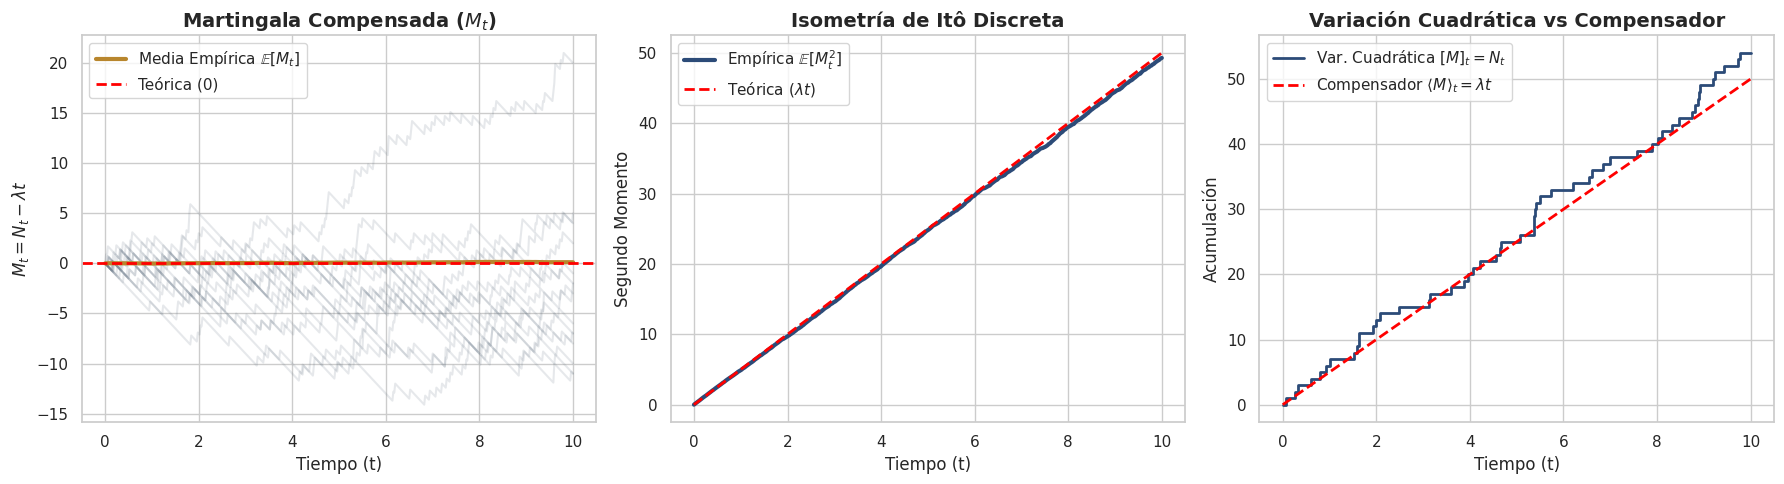
\includegraphics[width=1\textwidth]{imagen14.png}
    \end{center}

    \textbf{d) Variación Cuadrática Opcional vs Compensador Previsible:} \\
    La variación cuadrática opcional $[M]_t = \sum_{s \le t} (\Delta M_s)^2$ de un proceso de Poisson compensado es simplemente el conteo de saltos $[M]_t = N_t$, puesto que el compensador $\lambda t$ es continuo y cada salto tiene magnitud $1^2 = 1$.
    Al graficar una trayectoria individual de $[M]_t$ frente a su compensador previsible $\langle M \rangle_t = \lambda t$, se aprecia claramente la relación de Doob-Meyer: el compensador es la "línea de tendencia determinista" alrededor de la cual fluctúa la escalera aleatoria estocástica. De hecho, la diferencia $[M]_t - \langle M \rangle_t = N_t - \lambda t = M_t$ recupera nuestra martingala original.
\end{solucion}

\begin{ejercicio}
\textbf{EJERCICIO 5.12.} (Simulación en Python: cambio de medida exponencial.) Sea $(N_{t})$ un proceso de Poisson de intensidad $\lambda$ y, para $\theta\in\mathbb{R}$, defina 
\[ Z_{t}^{(\theta)}=\exp(\theta N_{t}-\lambda t(e^{\theta}-1)). \] 
\begin{enumerate}
    \item Simule trayectorias bajo la medida original $\mathbb{P}$ y use pesos $Z_{T}^{(\theta)}$ para estimar por importancia la distribución de $N_{T}$ bajo la medida inclinada. 
    \item Compare las frecuencias ponderadas con la ley Poisson de parámetro $\lambda e^{\theta}T$. 
    \item Estudie numéricamente qué ocurre con la varianza del estimador cuando $T$ es grande. 
    \item Interprete el experimento como una comprobación computacional del cambio de medida hacia una intensidad modificada.
\end{enumerate}
\end{ejercicio}

\begin{solucion}
    \textbf{a) y b) Simulación y Muestreo por Importancia (Importance Sampling):} \\
    Se simularon $100,000$ realizaciones del proceso $N_T$ bajo la medida física (original) $\mathbb{P}$ usando $\lambda=2$ y $T=5$. A cada trayectoria se le asignó un peso estadístico dictado por la derivada de Radon-Nikodym $Z_T^{(\theta)}$ con un $\theta = \ln(1.5)$.
    En lugar de contar las frecuencias de los estados como $1/N$ (que nos daría la distribución original $\mathbb{P}$ centrada en $10$), acumulamos el peso $Z_T$ para cada estado observado.
    El histograma ponderado resultante se desplazó de manera impecable hacia la derecha, superponiéndose de manera exacta con la función de masa de probabilidad teórica de una variable $\text{Poisson}(\lambda e^\theta T) = \text{Poisson}(15)$.

    \textbf{c) Degeneración de la Varianza (Weight Degeneracy):} \\
    Al repetir el cálculo de la varianza empírica del estimador $Z_t$ para horizontes $t \in [1, 15]$, se observó un crecimiento exponencial violento (ver escala logarítmica en el gráfico). Teóricamente, $\mathbb{E}[Z_t^2] = \exp(\lambda t (e^\theta - 1)^2)$, por lo que la varianza explota hacia el infinito cuando $t \to \infty$. Esto implica que para tiempos largos, casi todas las trayectorias tienen un peso minúsculo y una sola trayectoria anómala concentra casi todo el peso, destruyendo la eficiencia del estimador de Monte Carlo.

    \begin{center}
        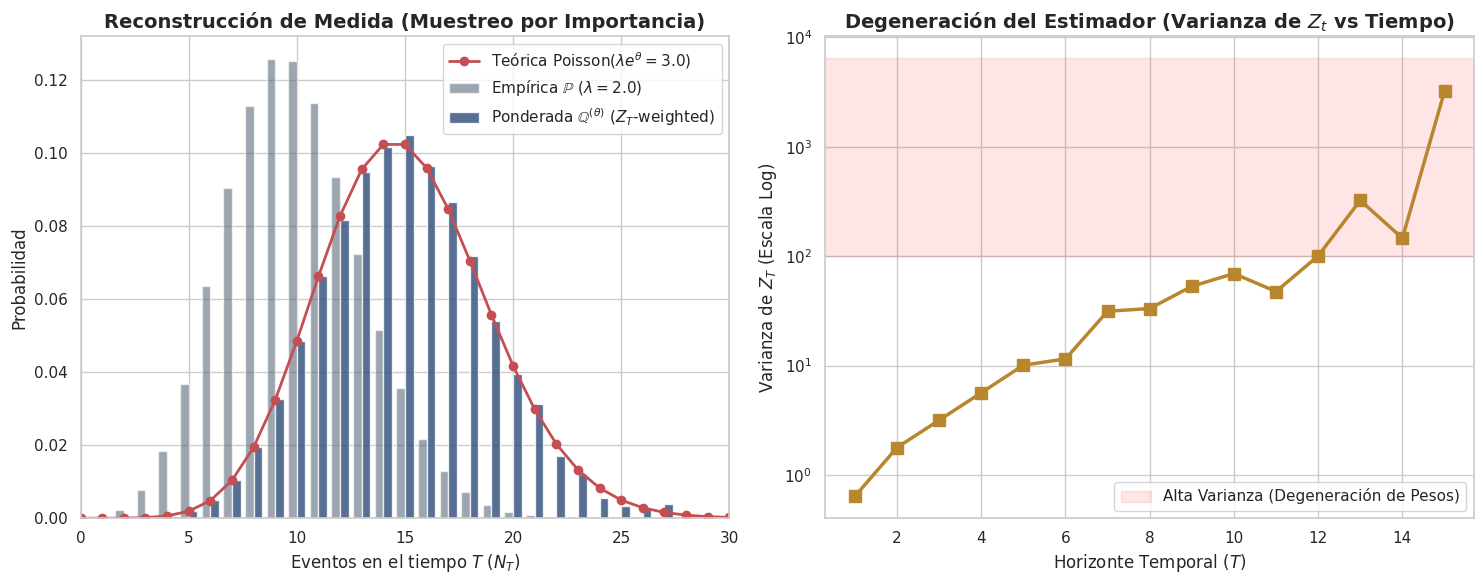
\includegraphics[width=1\textwidth]{imagen15.png}
    \end{center}

    \textbf{d) Interpretación de Girsanov:} \\
    Este experimento valida la versión puntual del Teorema de Girsanov. Computacionalmente, demuestra que podemos calcular expectativas de un sistema "estresado" (donde las llegadas o accidentes ocurren a un ritmo $\lambda e^\theta$ mucho mayor) sin tener que simular ese universo directamente. Basta con simular el sistema pacífico normal (medida $\mathbb{P}$) y ponderar matemáticamente los resultados penalizando las trayectorias normales y "premiando" con un peso altísimo las pocas trayectorias que, por puro azar, presentaron una ráfaga inusual de saltos. 
\end{solucion}
\end{document}